\documentclass[10pt,a4paper]{article}

\usepackage[a4paper,left=2.15cm,right=2.15cm,top=2.05cm,bottom=1.90cm,headheight=14pt,headsep=8pt,footskip=22pt]{geometry}
\usepackage[T1]{fontenc}
\usepackage[utf8]{inputenc}
\usepackage{lmodern}
\usepackage[authoryear,round]{natbib}
\usepackage[english]{babel}
\usepackage{microtype}
\usepackage{amsmath,amssymb,mathtools,amsthm,mathrsfs,bm}
\usepackage{booktabs,tabularx,array,multirow}
\usepackage{enumitem}
\usepackage{graphicx}
\usepackage{caption}
\usepackage{subcaption}
\usepackage{float}
\usepackage[most]{tcolorbox}
\usepackage{xcolor}
\usepackage{fancyhdr}
\usepackage{titlesec}
\usepackage{hyperref}
\usepackage{bookmark}

\definecolor{navy}{HTML}{153B5A}
\definecolor{teal}{HTML}{197A70}
\definecolor{ochre}{HTML}{B27612}
\definecolor{slate}{HTML}{5E7080}
\definecolor{paleblue}{HTML}{EDF3F6}
\definecolor{paleteal}{HTML}{EEF7F5}
\definecolor{paleochre}{HTML}{FBF5EA}

\hypersetup{
  colorlinks=true,
  linkcolor=navy,
  citecolor=teal,
  urlcolor=teal,
  pdftitle={Conditional Geometric Register of Observations: From Ridge to Feature Learning},
  pdfauthor={Redha Moulla},
  pdfsubject={Conditional invariants, observation diagnostics, nonlinear dynamics, and structural robustness},
  pdfkeywords={ridge, Tikhonov, observation, leverage, influence, Cook, Shapley, robustness, Jacobian, feature learning}
}

\pagestyle{fancy}
\fancyhf{}
\fancyhead[L]{\sffamily\small Conditional Geometric Register of Observations}
\fancyhead[R]{\sffamily\small Redha Moulla}
\fancyfoot[C]{\sffamily\small\thepage}
\renewcommand{\headrulewidth}{0.35pt}

\titleformat{\section}{\sffamily\bfseries\color{navy}\fontsize{15}{18}\selectfont}{\thesection}{0.72em}{}
\titlespacing*{\section}{0pt}{1.30ex plus .4ex minus .2ex}{0.55ex}
\titleformat{\subsection}{\sffamily\bfseries\color{navy}\fontsize{12.1}{14.3}\selectfont}{\thesubsection}{0.62em}{}
\titlespacing*{\subsection}{0pt}{1.05ex plus .35ex minus .2ex}{0.35ex}
\titleformat{\subsubsection}{\sffamily\bfseries\color{navy}\normalsize}{\thesubsubsection}{0.52em}{}
\titlespacing*{\subsubsection}{0pt}{0.9ex}{0.25ex}

\setlength{\parindent}{1.10em}
\setlength{\parskip}{0.05em}
\setlength{\abovedisplayskip}{7pt plus 2pt minus 2pt}
\setlength{\belowdisplayskip}{7pt plus 2pt minus 2pt}
\setlist[itemize]{leftmargin=1.7em,itemsep=0.20em,topsep=0.25em}
\setlist[enumerate]{leftmargin=2.0em,itemsep=0.24em,topsep=0.28em}
\captionsetup{font=small,labelfont=bf,justification=centering}

\newtcolorbox{abstractbox}{enhanced,breakable,colback=paleblue,colframe=navy,boxrule=0.8pt,arc=2.6mm,left=6mm,right=6mm,top=4.5mm,bottom=4.5mm}
\newtcolorbox{tealbox}[1][]{enhanced,breakable,colback=paleteal,colframe=teal,boxrule=0.75pt,arc=2mm,left=5mm,right=5mm,top=3mm,bottom=3mm,#1}
\newtcolorbox{ochrebox}[1][]{enhanced,breakable,colback=paleochre,colframe=ochre,boxrule=0.75pt,arc=2mm,left=5mm,right=5mm,top=3mm,bottom=3mm,#1}
\newtcolorbox{statementbox}[1]{enhanced,breakable,colback=white,colframe=teal,colbacktitle=teal,coltitle=white,fonttitle=\sffamily\bfseries,title={#1},boxrule=0.75pt,arc=1.5mm,left=5mm,right=5mm,top=3mm,bottom=3mm}
\newtcolorbox{resultbox}[1]{enhanced,breakable,colback=paleochre,colframe=ochre,colbacktitle=ochre,coltitle=white,fonttitle=\sffamily\bfseries,title={#1},boxrule=0.75pt,arc=1.5mm,left=5mm,right=5mm,top=3mm,bottom=3mm}

\newtheorem{theorem}{Theorem}[section]
\newtheorem{proposition}[theorem]{Proposition}
\newtheorem{corollary}[theorem]{Corollary}
\newtheorem{lemma}[theorem]{Lemma}
\newtheorem{definition}[theorem]{Definition}
\newtheorem{remark}[theorem]{Remark}
\renewcommand{\proofname}{Proof}

\newcommand{\R}{\mathbb{R}}
\newcommand{\E}{\mathbb{E}}
\newcommand{\Ker}{\operatorname{ker}}
\newcommand{\Img}{\operatorname{im}}
\newcommand{\rank}{\operatorname{rank}}
\newcommand{\tr}{\operatorname{tr}}
\newcommand{\diag}{\operatorname{diag}}
\newcommand{\spec}{\operatorname{spec}}
\newcommand{\Span}{\operatorname{span}}
\newcommand{\norm}[1]{\left\lVert #1\right\rVert}
\newcommand{\inner}[2]{\left\langle #1,#2\right\rangle}
\newcommand{\dd}{\mathrm d}
\newcommand{\Areg}{\mathscr A}
\newcommand{\Jreg}{\mathfrak D}
\newcommand{\Sigreg}{\mathfrak S}
\newcommand{\Qreg}{\mathscr Q}
\newcommand{\Id}{\mathrm I}

\begin{document}
\hypersetup{pageanchor=false}

% -----------------------------------------------------------------------------
% Cover
% -----------------------------------------------------------------------------
\thispagestyle{empty}
\vspace*{1.25cm}
{\sffamily\color{teal}\fontsize{11.5}{14}\selectfont WORKING PAPER -- VERSION 7 -- AUGUST 2026\par}
\vspace{0.95cm}
{\sffamily\bfseries\color{black!88}\fontsize{24.5}{29}\selectfont Conditional Geometric Register\\of Observations\par}
\vspace{0.28cm}
{\sffamily\color{slate}\fontsize{16.2}{19}\selectfont From Ridge to Feature Learning: Invariants, Diagnostics, and Dynamics\par}
\vspace{0.22cm}
{\sffamily\bfseries\color{teal}\fontsize{11.2}{14}\selectfont Observation Qualification and Structural Robustness\par}
\vspace{0.68cm}
{\sffamily\fontsize{12}{14}\selectfont Redha Moulla\par}
{\sffamily\small\color{slate} AXIA, France\par}
\vspace{0.60cm}

\begin{abstractbox}
\small
\textbf{Abstract.} A training observation acts simultaneously on model observability and on the model state. Relative to a context $S$, we describe it by the decorated Gauss--Newton quadratic datum
\[
\Jreg_{i\mid S}=(G_S,\Gamma_i,\alpha_i),
\]
where $G_S\succ0$ is the collective geometry, $\Gamma_i\succeq0$ is the observability increment, and $\alpha_i$ is the cotangent effort. After whitening, this datum becomes a pair $(B,b)$ defined modulo an orthogonal action. Its orbit is completely classified by the spectrum of $B$ and by the energy of $b$ in each eigenspace. The principal quotient admits a global chart with $2p$ coordinates, but an isolated observation most often lies on a low-rank stratum: for $\rank B=r<p$, the generic stratum has $2r+1$ invariants, and $2r$ when the effort is compatible with the curvature, $b\in\Img B$. The scalar quadratic case therefore corresponds to $r=1$ and reduces exactly to conditional leverage and the magnitude of the studentized innovation. Leverage, information gain, Cook's distance, target influence, and marginal information contributions appear as non-injective scalarizations of the register; genuinely non-scalar structure becomes possible as soon as the rank exceeds one.

The triplet is complete only for the parametric action of the Gauss--Newton quadratic model, up to an additive constant. We further distinguish invisibility induced by the loss metric from invisibility induced by the parametric pullback, without assuming that their projectors commute. In the nonlinear setting, finite insertion follows a reweighting path along which observability and effort evolve. The experiments verify the exact identities, exhibit a collision of five scalarizations in rank three, and track the functional mobility of a network. Public and private tabular stress tests then illustrate contraction and innovation budgets, together with their nominal costs and transfer limitations. This robust prototype remains secondary and is not claimed as novel: the main contribution is the non-scalar, stratified classification of the conditional action of an observation before any scalar attribution.
\end{abstractbox}

\clearpage
\hypersetup{pageanchor=true}
\pagenumbering{arabic}
\setcounter{tocdepth}{1}
\tableofcontents
\clearpage

% -----------------------------------------------------------------------------
\section{Introduction}
% -----------------------------------------------------------------------------
Data valuation and diagnostic methods often ask an apparently simple question: \emph{how much is an observation worth?} Leverage, studentized residuals, Cook's distance, influence functions, information gain, leave-one-out, and Data Shapley provide different answers because they do not measure the same effect. An observation may reveal a direction that was previously poorly determined, strongly contradict the model, move the parameters without changing a given target, or contribute to a utility only in certain contexts. Reducing these effects to a single number is useful for ranking points, but it destroys part of their structure.

The starting point of this paper is the contraction--displacement law already visible in Ridge. A scalar observation $y=h^\top\theta+\varepsilon$ adds the positive tensor $hh^\top/r$ to the precision, contracts the covariance along the dual direction $Ph$, and its innovation then moves the estimator along that same direction. In the nonlinear setting, $h^\top$ is replaced by the Jacobian $J_i(\theta)$; the directions of observability then depend on the current point and may evolve with the representations.

The first objective is to identify the object upstream of scalar diagnostics. To a context $S$ and an observation $i$, we associate the relative quadratic datum
\[
\Jreg_{i\mid S}=(G_S,\Gamma_i,\alpha_i),
\]
where the separation between the context geometry $G_S$ and the point-specific increment $\Gamma_i$ is retained. After choosing a $G_S$-orthonormal frame, the intrinsic information is the orthogonal orbit of $(B,b)$. Its complete signature contains the eigenvalues of $B$, their multiplicities, and the energy of $b$ in each eigenspace. This classification is a finite-dimensional specialization of classical results from spectral theory and orthogonal invariants; the contribution of the paper lies in applying it to the conditional qualification of an observation.

The second objective is to state precisely what is meant by \emph{factorization}. The result does not concern the total quadratic function alone: it concerns the \emph{decorated} datum $(G_S,\Gamma_i,\alpha_i)$, whose context--observation decomposition is part of the object. In a fixed additive geometry, classical diagnostics are non-injective maps of this register: traces, log-determinants, norms, pairings with a target, or averages over contexts. In a fully retrained nonlinear model, additivity is replaced by a reweighting path.

The third objective is practical: to separate qualification from decision. The register may indicate that a point is geometrically novel, locally discordant, highly influential, or structurally invalid. It does not follow that a single loss weight is optimal. Contraction and innovation budgets are presented as one admission policy within the family of GM-estimators, not as a new universal estimator.

\begin{statementbox}{Contributions of version 7}
\begin{enumerate}
  \item A relative quadratic datum $(G_S,\Gamma_i,\alpha_i)$ whose scope is explicitly limited to the parametric action of the local Gauss--Newton model, up to an additive constant.
  \item A complete orbit classification of the whitened pair $(B,b)$, a global diffeomorphism for the principal quotient, and an explicit classification of generic rank-$r$ strata, of dimensions $2r+1$ or $2r$ under the compatibility condition $b\in\Img B$.
  \item An effort--curvature compatibility lemma showing that $W_i\succ0$ implies $\alpha_i\in\Img\Gamma_i$, which naturally places scalar quadratic observations on the compatible rank-one stratum.
  \item A separation between invisibility in loss curvature, $\Ker(W_ih_i^\sharp)$, and parametric invisibility, $\Ker J_i^*$, together with the observation that these marginal diagnostics may overlap.
  \item An exact factorization of classical diagnostics, a simultaneous collision of five scalarizations constructed in rank three, and extensions to multiple targets and nonlinear trajectories.
  \item Tightened robustness controls: an identifier-level internal SeLoger holdout, a Huber baseline with a non-geometric scale, sensitivity of $\kappa_X$ to listing mass, and a public replication on Concrete Compressive Strength.
  \item Broader positioning relative to the Memory--Perturbation Equation, the Versatile Influence Function, and singular Riemannian geometries for neural networks.
\end{enumerate}
\end{statementbox}

The contribution is not the invention of leverage, influence, Fisher geometry, Shapley values, spectral classification, or robust estimators. It is the structured application of these invariants to a non-scalar conditional datum for each observation, followed by a precise identification of what is lost under scalarization.

% -----------------------------------------------------------------------------
\section{Preliminaries: Observation, Quotient, and Contraction}
% -----------------------------------------------------------------------------
\subsection{Linear semi-geometry}
Let $\Theta=\R^p$, $Y=\R^n$, $A:\Theta\to Y$, and
\[
y=A\theta^\star+\varepsilon,\qquad \E[\varepsilon]=0,\qquad \operatorname{Cov}(\varepsilon)=R\succ0.
\]
The weighted quadratic loss is
\begin{equation}
L(\theta)=\frac12\norm{A\theta-y}_{R^{-1}}^2,
\qquad
G_A=A^\top R^{-1}A.
\end{equation}
For every $u$,
\[
u^\top G_Au=\norm{Au}_{R^{-1}}^2,
\]
so $\Ker G_A=\Ker A$. The form is degenerate on $\Theta$ when $A$ is not injective, but it becomes a non-degenerate metric on the identifiable quotient $\Theta/\Ker A$. The geometry is constant and flat on this quotient; it is not a non-degenerate Riemannian metric on all of $\Theta$.

The weighted Moore--Penrose pseudoinverse does not reconstruct any component in $\Ker A$ \citep{penrose1955}. It resolves the non-uniqueness caused by this kernel by selecting the representative of minimum $M$-norm:
\begin{equation}
\theta_M^\dagger
=
\theta_0+M^{-1/2}\bigl(R^{-1/2}AM^{-1/2}\bigr)^\dagger R^{-1/2}(y-A\theta_0),
\qquad M\succ0.
\end{equation}
A complete proof is given in Appendix~\ref{app:pseudoinverse}.

\subsection{Tikhonov regularization and the soft kernel}
Tikhonov regularization, of which Ridge is the classical statistical form \citep{tikhonov1963,hoerl1970}, is
\begin{equation}
E_\lambda(\theta)
=
\frac12\norm{A\theta-y}_{R^{-1}}^2
+
\frac\lambda2\norm{\theta-\theta_0}_M^2
\end{equation}
and adds a reference geometry:
\[
G_\lambda=A^\top R^{-1}A+\lambda M\succ0.
\]
The minimizer is unique and converges, as $\lambda\downarrow0$, to $\theta_M^\dagger$. In whitened coordinates, the components are filtered by $\sigma_j/(\sigma_j^2+\lambda)$. The pseudoinverse addresses exact non-uniqueness; Ridge damps directions that are nonzero but insufficiently resolved. The operator
\begin{equation}
N_\lambda=\lambda(G_A+\lambda I)^{-1}
\end{equation}
has eigenvalues $\lambda/(\mu_j+\lambda)$ and measures continuous residual non-identifiability. Its boundary depends on noise, the reference metric, and the target risk; it cannot be inferred from the algebraic kernel alone.

\subsection{An observation increases precision and contracts uncertainty}
Consider a scalar observation
\[
y_i=h_i^\top\theta+\varepsilon_i,\qquad \operatorname{Var}(\varepsilon_i)=r_i>0.
\]
Under the exact Bayesian interpretation, we assume a Gaussian prior and conditionally independent Gaussian noise. With
\[
P^-=(G_S)^{-1},\qquad s_i=h_i^\top P^-h_i,
\qquad S_i=r_i+s_i,
\qquad \nu_i=y_i-h_i^\top\widehat\theta_S,
\]
the Sherman--Morrison identity \citep{sherman1950} gives
\begin{align}
P^+&=P^--\frac{P^-h_ih_i^\top P^-}{S_i},\label{eq:cov-update}\\
\widehat\theta_{S+i}-\widehat\theta_S
&=\frac{P^-h_i}{S_i}\nu_i.\label{eq:mean-update}
\end{align}
Thus covariance or uncertainty contracts, while precision and information increase. The image of $P^--P^+$ and the displacement both belong to $\Span(P^-h_i)$. Without Gaussianity, the same identities describe recursive Ridge or recursive least squares, but $P$ is no longer automatically an exact posterior covariance \citep{kalman1960,ollivier2017}.

\subsection{Cotangent effort and displacement}
For a smooth map $F:\Theta\to Y$, its differential $J_\theta=\dd F_\theta$ maps parametric tangent vectors to output variations. The loss provides an output covector $e_y=\dd_1\ell(F(\theta),y)$, pulled back as
\[
\alpha_\theta=J_\theta^*e_y\in T_\theta^*\Theta.
\]
A metric $g_\theta$ converts this effort into motion:
\begin{equation}
\dot\theta=-g_\theta^\sharp\alpha_\theta,
\qquad
\dot F=-J_\theta g_\theta^\sharp J_\theta^*e_y.
\end{equation}
Ordinary gradient, natural gradient, and Gauss--Newton steps differ through the cometric they use \citep{amari1998,ollivier2015,martens2020}. Dissipation is metric: under gradient flow, $\dd E/\dd t=-\norm{\operatorname{grad}_gE}_g^2\leq0$. If momentum is introduced, a correct mechanical formulation uses an independent mass matrix
\[
H(\theta,p)=\frac12p^\top M_{\rm kin}^{-1}p+E(\theta),\qquad M_{\rm kin}\succ0,
\]
rather than the inverse of a possibly rectangular design matrix.

\subsection{Local nonlinear geometry}
For a sample $S$, let $F_S(\theta)=(f_\theta(x_j))_{j\in S}$ and $J_S(\theta)=\dd F_S|_\theta$. A positive output metric $W_S$ induces
\begin{equation}
G_S^{\rm obs}(\theta)=G_0(\theta)+J_S(\theta)^*W_S(\theta)J_S(\theta).
\end{equation}
The tangent kernel is $\Ker J_S(\theta)$. If the rank is constant, it is tangent to the local fibers of $F_S$; if the rank varies, the geometry is stratified. For a general loss, $W_i=\dd_1^2\ell_i$ may depend on the label. The separation ``inputs construct, labels localize'' is therefore exact only when the output metric is label-independent: quadratic loss, certain canonical families, or an explicitly chosen conditional Fisher metric.

The exact Hessian of the loss is not, in general, equal to $G_S^{\rm obs}$:
\[
H_S=G_S^{\rm obs}+\text{second-order model terms}.
\]
This distinction will be central to nonlinear influence. Damped Levenberg--Marquardt local models stabilize the inversion of precisely this tangent geometry \citep{levenberg1944,marquardt1963,marquardt1970}.

% -----------------------------------------------------------------------------
\section{Relative Quadratic Datum and Complete Orbit Signature}
% -----------------------------------------------------------------------------
\subsection{Local definition and scope}
Fix a point $\widehat\theta_S$ that minimizes the context loss for $S$. In the tangent space $V=T_{\widehat\theta_S}\Theta$, assume a positive-definite geometry $G_S:V\to V^*$, denoted $G_S\succ0$, and, for observation $i$,
\begin{equation}
\alpha_i=\dd\ell_i|_{\widehat\theta_S}\in V^*,
\qquad
\Gamma_i=J_i^*W_iJ_i:V\to V^*,
\qquad \Gamma_i\succeq0.
\end{equation}
The quadratic insertion model is
\begin{equation}
Q_{i\mid S}(\delta)
=
\frac12\inner{\delta}{G_S\delta}
+
\inner{\alpha_i}{\delta}
+
\frac12\inner{\delta}{\Gamma_i\delta}.
\label{eq:local-quadratic-model}
\end{equation}

\begin{definition}[Relative quadratic observation datum]
The \emph{relative quadratic datum} of point $i$ in context $S$ is the decorated triplet
\begin{equation}
\boxed{\Jreg_{i\mid S}=(G_S,\Gamma_i,\alpha_i).}
\label{eq:decorated-relative-data}
\end{equation}
The separation between the collective geometry $G_S$ and the point-specific increment $\Gamma_i$ is part of the object.
\end{definition}

\begin{remark}[Why we no longer use the term ``2-jet'']
A second-order jet in the standard sense contains the value, first order, and full second order of a map, together with the transformation laws of jet bundles \citep{saunders1989}. The triplet \eqref{eq:decorated-relative-data} contains neither the value $\ell_i(\widehat\theta_S)$ nor the exact Hessian of $\ell_i$, and $G_S$ belongs to the context. It is therefore a Gauss--Newton datum decorated by the context, not a second-order jet in the usual geometric sense.
\end{remark}

Setting $P_S=G_S^{-1}$, the derived practical objects are
\begin{equation}
R_{i\mid S}=P_S\Gamma_i,
\qquad
C_{i\mid S}=R_{i\mid S}(I+R_{i\mid S})^{-1},
\label{eq:R-C}
\end{equation}
\begin{equation}
v_{i\mid S}^{\rm obs}=-P_S\alpha_i,
\qquad
d_{i\mid S}^{\rm obs}=-(G_S+\Gamma_i)^{-1}\alpha_i.
\label{eq:v-d}
\end{equation}
The first vector is the infinitesimal response of the local Gauss--Newton model; the second is its finite minimizer. They are the exact statistical influence only when $G_S$ coincides with the exact Hessian of the context.

\begin{remark}[Overcomplete practical register, loss constant, and output information]
The register
\[
\Areg_{i\mid S}
=(\Gamma_i,\alpha_i,R_{i\mid S},C_{i\mid S},v_{i\mid S}^{\rm obs},d_{i\mid S}^{\rm obs})
\]
is deliberately overcomplete. Its generator remains $\Jreg_{i\mid S}$. The latter is complete for the \emph{parametric action of the declared Gauss--Newton quadratic model, up to an additive constant}. A utility that depends on the absolute loss value additionally requires
\[
c_i=\ell_i(\widehat\theta_S).
\]
This scalar belongs to the extended passport, but not to the tensorial core of the register.

The register does not contain the entire output error. Two distinct forms of invisibility must be separated. First, if $W_i:T_yY_i\to T_y^*Y_i$ is singular, choose an auxiliary metric
\[
h_i^\flat:T_yY_i\longrightarrow T_y^*Y_i,
\qquad h_i^\sharp=(h_i^\flat)^{-1},
\]
and set
\[
\widetilde W_i=W_i h_i^\sharp:T_y^*Y_i\longrightarrow T_y^*Y_i.
\]
The endomorphism $\widetilde W_i$ is self-adjoint with respect to the dual metric induced by $h_i$. Consequently,
\[
T_y^*Y_i=\Img\widetilde W_i\oplus^{\perp_{h_i^{-1}}}\Ker\widetilde W_i,
\]
and
\[
e_i=e_i^{\rm loss,1}+e_i^{\rm loss,0},
\qquad
e_i^{\rm loss,1}\in\Img\widetilde W_i,
\quad
e_i^{\rm loss,0}\in\Ker\widetilde W_i.
\]
The component visible to the loss curvature can be measured by
\[
\norm{e_i^{\rm loss,1}}_{W_{i,h}^{\dagger}}^2
=\inner{e_i^{\rm loss,1}}{W_{i,h}^{\dagger}e_i^{\rm loss,1}},
\]
where $W_{i,h}^{\dagger}:T_y^*Y_i\to T_yY_i$ is the pseudoinverse defined relative to $h_i$.

Second, parametric invisibility is governed by
\[
\Ker J_i^*\subset T_y^*Y_i.
\]
It is independent of the previous notion: a covector may be well measured by $W_i$ yet annihilated by the pullback. We therefore also retain
\[
\boxed{
 e_i^{\rm par,0}
 =\Pi_{\Ker J_i^*}^{\,h_i^{-1}}e_i,
 \qquad
 e_i^{\rm par,1}=e_i-e_i^{\rm par,0}.
}
\]
Only $e_i^{\rm par,1}$ contributes to $\alpha_i=J_i^*e_i$. The extended passport may therefore report $c_i$, $e_i^{\rm loss,0}$, and $e_i^{\rm par,0}$ separately. The projectors $\Pi_{\Ker\widetilde W_i}$ and $\Pi_{\Ker J_i^*}$ do not generally commute, however. The two invisible components are therefore overlapping marginal diagnostics, not terms in a common orthogonal partition of the error; their norms must not be added as a variance decomposition. If $W_i\succ0$, one may simply use $\norm{e_i}_{W_i^{-1}}$; an independent audit metric $H_i\succ0$ is also possible.
\end{remark}

\subsection{Reparameterization, whitening isometry, and orbit}
Under a local coordinate change $\theta'=\varphi(\theta)$ with invertible differential $A=\dd\varphi_\theta$, the objects transform as
\begin{equation}
G_S'=A^{-\top}G_SA^{-1},
\qquad
\Gamma_i'=A^{-\top}\Gamma_iA^{-1},
\qquad
\alpha_i'=A^{-\top}\alpha_i.
\label{eq:covariance-laws}
\end{equation}
Consequently, $R$ and $C$ transform by similarity, whereas $v$ and $d$ transform as tangent vectors.

Choose an isometry
\[
L:(V,G_S)\longrightarrow(\R^p,I).
\]
In this $G_S$-orthonormal frame, the datum becomes
\begin{equation}
B=L^{-\top}\Gamma_iL^{-1}\succeq0,
\qquad
b=L^{-\top}\alpha_i.
\label{eq:whitened-pair}
\end{equation}
In Euclidean coordinates with $L=G_S^{1/2}$, this reads $B=G_S^{-1/2}\Gamma_iG_S^{-1/2}$ and $b=G_S^{-1/2}\alpha_i$. Two whitening isometries differ by some $Q\in O(p)$ and transform
\begin{equation}
(B,b)\longmapsto(QBQ^\top,Qb).
\end{equation}
The intrinsic object is therefore the orthogonal orbit $[B,b]$.

\begin{definition}[Orbit signature]
Let $\lambda$ be a distinct eigenvalue of $B$, with multiplicity $m_\lambda$, and let $\Pi_\lambda$ be the orthogonal projector onto its eigenspace. We define
\begin{equation}
\boxed{
\Sigreg(B,b)
=
\bigl\{(\lambda,m_\lambda,\beta_\lambda):
\beta_\lambda=\norm{\Pi_\lambda b}^2\bigr\}_{\lambda\in\spec(B)}.
}
\label{eq:orbital-signature}
\end{equation}
\end{definition}

The following classification is a finite-dimensional consequence of the spectral theory of a self-adjoint operator and the action of its orthogonal stabilizer; it is not claimed as a new abstract theorem \citep{halmos1951,weyl1946,sibirskii1967,sibirskii1968,khadzhiev1967}. We state it explicitly to characterize the intrinsic information carried by the observation.

\begin{theorem}[Complete orbit classification]
Two whitened pairs $(B,b)$ and $(B',b')$ are related by an orthogonal transformation
\[
B'=QBQ^\top,
\qquad
b'=Qb
\]
if and only if their orbit signatures \eqref{eq:orbital-signature} coincide.
\label{thm:orbit-classification}
\end{theorem}

\begin{proof}
Necessity is immediate. Conversely, for each eigenvalue $\lambda$, the eigenspaces $E_\lambda$ and $E'_\lambda$ have the same dimension, and the vectors $\Pi_\lambda b$ and $\Pi'_\lambda b'$ have the same norm. The group $O(E_\lambda)$ acts transitively on each sphere, so there is an isometry $Q_\lambda:E_\lambda\to E'_\lambda$ mapping one vector to the other. The orthogonal direct sum $Q=\bigoplus_\lambda Q_\lambda$ satisfies both identities.
\end{proof}

\begin{proposition}[Principal quotient and global coordinates]
Let
\[
\mathcal P=
\left\{(B,b)\in\operatorname{Sym}_{++}(p)\times\R^p:
\lambda_1(B)<\cdots<\lambda_p(B),\ 
\langle b,e_j(B)\rangle\neq0\ \forall j
\right\}.
\]
The action of $O(p)$ on $\mathcal P$ is free. The map
\[
\Phi:\mathcal P/O(p)\longrightarrow
\Lambda_p\times(\R_{>0})^p,
\qquad
[B,b]\longmapsto
(\lambda_1,\ldots,\lambda_p,\beta_1,\ldots,\beta_p),
\]
where
\[
\Lambda_p=\{(\lambda_1,\ldots,\lambda_p):0<\lambda_1<\cdots<\lambda_p\},
\qquad
\beta_j=\langle b,e_j(B)\rangle^2,
\]
is a global diffeomorphism. The principal quotient is therefore a manifold of dimension $2p$.
\label{prop:principal-quotient}
\end{proposition}
\begin{proof}
If $Q\in O(p)$ stabilizes $(B,b)$, then $QB=BQ$. Since the spectrum of $B$ is simple, in the ordered eigenbasis one has $Qe_j=\varepsilon_je_j$ with $\varepsilon_j\in\{-1,1\}$. The equality $Qb=b$ and the non-vanishing of every component of $b$ force $\varepsilon_j=1$ for all $j$; hence the stabilizer is trivial.

The ordered signature is constant on orbits. Conversely, every orbit has a representative of the form
\[
B=\diag(\lambda_1,\ldots,\lambda_p),
\qquad
b=(\sqrt{\beta_1},\ldots,\sqrt{\beta_p})^\top,
\]
obtained by ordering the eigenvectors and choosing their signs so that the components of $b$ are positive. This representative is unique. The explicit inverse map
\[
(\lambda,\beta)\longmapsto
\left[\diag(\lambda_1,\ldots,\lambda_p),
(\sqrt{\beta_1},\ldots,\sqrt{\beta_p})^\top\right]
\]
is smooth, as is $\Phi$ on the simple-spectrum stratum. This proves the stated diffeomorphism.
\end{proof}

\begin{corollary}[Minimum dimension of a regular local representation]
Let $U$ be an open subset of the principal quotient and let $f:U\to\R^k$ be a smooth locally injective map whose differential is injective at every point, that is, a locally injective immersion. Then $k\ge 2p$.
\end{corollary}
\begin{proof}
By Proposition~\ref{prop:principal-quotient}, $U$ is a manifold of dimension $2p$. Injectivity of $\dd f$ implies $\rank(\dd f)=2p$, hence $k\ge2p$.
\end{proof}

\begin{remark}
The principal quotient is a useful reference stratum, but it is rarely the application-relevant stratum of an isolated observation:
\[
\rank\Gamma_i\leq\dim Y_i.
\]
A scalar observation therefore has an increment of rank at most one, regardless of the number of parameters. Low-rank strata are treated below; repeated positive eigenvalues and zero spectral energies form lower-dimensional boundaries, still classified by the complete signature of Theorem~\ref{thm:orbit-classification}.
\end{remark}

\subsection{Generic low-rank strata}
Let $1\leq r<p$ and $q=p-r$. We consider pairs $(B,b)$ such that $B\succeq0$ has exactly $r$ simple positive eigenvalues
\[
0<\lambda_1<\cdots<\lambda_r,
\]
a kernel $E_0=\Ker B$ of dimension $q$, and energies
\[
\beta_j=\norm{\Pi_{\lambda_j}b}^2>0,
\qquad
\beta_0=\norm{\Pi_0b}^2>0.
\]

\begin{proposition}[Generic rank-$r$ stratum]
On this stratum, the orbit space under $O(p)$ is globally parameterized by
\begin{equation}
\boxed{
(\lambda_1,\ldots,\lambda_r,
 \beta_1,\ldots,\beta_r,\beta_0)
\in
\Lambda_r\times(\R_{>0})^{r+1},
}
\label{eq:rank-r-stratum}
\end{equation}
where $\Lambda_r=\{0<\lambda_1<\cdots<\lambda_r\}$. It therefore has dimension $2r+1$. Every orbit admits the canonical representative
\begin{equation}
B=\diag(\lambda_1,\ldots,\lambda_r,0,\ldots,0),
\qquad
b=(\sqrt{\beta_1},\ldots,\sqrt{\beta_r},\sqrt{\beta_0},0,\ldots,0)^\top.
\label{eq:rank-r-canonical}
\end{equation}
\label{prop:rank-r-stratum}
\end{proposition}

\begin{proof}
Theorem~\ref{thm:orbit-classification} already shows that the quantities in \eqref{eq:rank-r-stratum} classify the orbits. Conversely, order the positive eigenspaces, choose the sign of each eigenvector so that the corresponding component of $b$ is positive, and use the transitive action of $O(E_0)$ on the sphere of radius $\sqrt{\beta_0}$ to align the kernel component with the first axis of $E_0$. This yields \eqref{eq:rank-r-canonical}, unique modulo the stabilizer $O(q-1)$ acting on the orthogonal complement of this component without changing the pair. The canonical section and the invariants identify the orbit space globally with the domain in \eqref{eq:rank-r-stratum}.
\end{proof}

The component $\beta_0$ measures a first-order effort in a direction along which the observation supplies no Gauss--Newton curvature. It is therefore not a merely algebraic detail: it distinguishes an effort compatible with quadratic observability from an effort carried by the kernel of $B$.

\begin{corollary}[Compatible stratum]
Under the additional assumption
\[
b\in\Img B,
\]
one has $\beta_0=0$. The generic compatible stratum is globally parameterized by
\[
(\lambda_1,\ldots,\lambda_r,
 \beta_1,\ldots,\beta_r)
\in\Lambda_r\times(\R_{>0})^r
\]
and has dimension $2r$.
\label{cor:compatible-stratum}
\end{corollary}

\begin{lemma}[Effort--curvature compatibility]
In finite dimension, if $W_i\succ0$, then
\begin{equation}
\boxed{
\alpha_i=J_i^*e_i\in\Img\Gamma_i,
\qquad
\Gamma_i=J_i^*W_iJ_i.
}
\label{eq:compatibility-lemma}
\end{equation}
More generally, if $W_i\succeq0$ and $e_i\in\Img W_i$, the same conclusion holds. After whitening, $b\in\Img B$.
\label{lem:effort-curvature-compatibility}
\end{lemma}

\begin{proof}
If $W_i\succ0$, then $\Ker\Gamma_i=\Ker J_i$. For a positive self-adjoint operator in finite dimension,
\[
\Img\Gamma_i=(\Ker\Gamma_i)^\circ,
\]
whereas $\Img J_i^*=(\Ker J_i)^\circ$. Hence $\Img\Gamma_i=\Img J_i^*$, and $\alpha_i=J_i^*e_i$ belongs to this image. If $W_i\succeq0$ and $e_i=W_iu$, set $A=W_i^{1/2}J_i$ in a declared auxiliary metric. Then $\Gamma_i=A^*A$ and $\alpha_i=A^*W_i^{1/2}u$. Since $\Img(A^*A)=\Img A^*$ in finite dimension, the result follows. Whitening is an isomorphism and preserves membership in the corresponding images.
\end{proof}

\begin{remark}[Scalar case]
For a non-degenerate scalar quadratic observation, $r\leq1$ and Lemma~\ref{lem:effort-curvature-compatibility} forces the compatible stratum. When $r=1$, the quotient therefore has exactly two parameters. The recovery result in Section~\ref{subsec:rankone-recovery} will show that they can be chosen as the conditional leverage $\rho_i$ and the magnitude of the studentized innovation $|z_i|$. Thus the $2p$-parameter principal quotient is not the relevant case for a scalar observation: it serves as a reference stratum for the general theorem, whereas the low-rank stratum is the dominant applied case.
\end{remark}

\subsection{Quotient property and the role of decoration}
\begin{corollary}[Factorization of invariant diagnostics]
Let $F$ be a function of the decorated relative quadratic datum $(G,\Gamma,\alpha)$ that is constant under the reparameterization laws \eqref{eq:covariance-laws}. Then there exists a unique function $\bar F$ defined on the \emph{image} of the signature such that
\begin{equation}
F(G,\Gamma,\alpha)
=\bar F\bigl(\Sigreg(L^{-\top}\Gamma L^{-1},L^{-\top}\alpha)\bigr),
\end{equation}
where $L:(V,G)\to(\R^p,I)$ is any isometry.
\end{corollary}
\begin{proof}
After whitening, invariance means that $F$ is constant on orthogonal orbits. Theorem~\ref{thm:orbit-classification} identifies these orbits with the fibers of $\Sigreg$. The universal property of the quotient defines $\bar F$ on the image of the signature and ensures uniqueness there.
\end{proof}

\begin{remark}[The total quadratic function is not sufficient]
The decoration $(G,\Gamma,\alpha)$ is essential. In dimension one, $(G_1,\Gamma_1,\alpha_1)=(1,1,0)$ and $(G_2,\Gamma_2,\alpha_2)=(3/2,1/2,0)$ define the same total function $Q(\delta)=\delta^2$, but their whitened ratios are $B_1=1$ and $B_2=1/3$, so their relative contractions are respectively $1/2$ and $1/4$. The register distinguishes the geometry already acquired from the information added by the point.
\end{remark}

\subsection{Derived tensorial register}
In a whitened frame,
\begin{equation}
\bar C=B(I+B)^{-1},
\qquad
\bar v=-b,
\qquad
\bar d=-(I+B)^{-1}b.
\label{eq:canonical-register}
\end{equation}
The signature reconstructs their \emph{orbits}, spectra, energies by eigenspace, and all invariant scalarizations; it does not reconstruct a particular oriented vector in the original tangent space. Displaying a parametric direction requires retaining a representative of $(G,\Gamma,\alpha)$.

Several common scalarizations are
\begin{align}
\tr \bar C
&=\sum_\lambda m_\lambda\frac{\lambda}{1+\lambda},\label{eq:traceC}\\
\mathcal I
&=\frac12\log\det(I+B)
=\frac12\sum_\lambda m_\lambda\log(1+\lambda),\label{eq:infoB}\\
\norm{\bar v}^2
&=\sum_\lambda\beta_\lambda,\label{eq:normv}\\
\norm{\bar d}^2
&=\sum_\lambda\frac{\beta_\lambda}{(1+\lambda)^2},\label{eq:normd}\\
\norm{\bar d}_{I+B}^2
&=\sum_\lambda\frac{\beta_\lambda}{1+\lambda}.\label{eq:postnormd}
\end{align}
These maps are non-injective: they aggregate the spectrum or the distribution of effort.

\subsection{Multiple targets: spectral Gram matrices}
Influence on a target $\tau$ requires the whitened covector $t=L^{-\top}\dd\tau$. For $k$ targets $t_1,\dots,t_k$, define in each eigenspace
\[
Z_\lambda=
\bigl[\Pi_\lambda b,\Pi_\lambda t_1,\dots,\Pi_\lambda t_k\bigr],
\qquad
\mathcal G_\lambda=Z_\lambda^\top Z_\lambda.
\]

\begin{theorem}[Classification with targets]
The orbit of $(B,b,t_1,\dots,t_k)$ under the joint orthogonal action is completely characterized by
\begin{equation}
\bigl\{(\lambda,m_\lambda,\mathcal G_\lambda)\bigr\}_{\lambda\in\spec(B)}.
\label{eq:target-signature}
\end{equation}
\end{theorem}
\begin{proof}
Within each eigenspace, two finite families of vectors are related by an orthogonal isometry if and only if their Gram matrices coincide. Construct these isometries eigenspace by eigenspace, then take their orthogonal direct sum.
\end{proof}
For a single target, the $2\times2$ matrix retains $\norm{\Pi_\lambda b}^2$, $\norm{\Pi_\lambda t}^2$, and their signed cross-product. It therefore recovers $t^\top\bar v$ or $t^\top\bar d$ without losing relative orientation.

\subsection{Composition limit across observations}
The signature classifies an observation \emph{in a fixed context}. It is not sufficient to reconstruct the relative angles among several prospective observations. With $G=I_2$ and zero efforts, the families
\[
B_1=e_1e_1^\top,\quad B_2=e_1e_1^\top
\qquad\text{and}\qquad
B'_1=e_1e_1^\top,\quad B'_2=e_2e_2^\top
\]
have the same individual signatures, but
\[
B_1+B_2=\diag(2,0),
\qquad
B'_1+B'_2=I_2.
\]
Experimental design, joint selection, and redundancy among points therefore require the tensors in a common frame or simultaneous invariants; they cannot be recovered from the collection of individual signatures alone.

% -----------------------------------------------------------------------------
\section{Recovering Diagnostics in a Frozen Geometry}
% -----------------------------------------------------------------------------
\subsection{Scalar linear rank-one case}
\label{subsec:rankone-recovery}
Consider again an observation $y_i=h_i^\top\theta+\varepsilon_i$ with variance $r_i$, added after a context with geometry $G_S\succ0$ and estimator $\widehat\theta_S$. Define
\begin{equation}
s_i=h_i^\top P_Sh_i,
\qquad
q_i=\frac{s_i}{r_i},
\qquad
\nu_i=y_i-h_i^\top\widehat\theta_S,
\qquad
z_i=\frac{\nu_i}{\sqrt{r_i+s_i}},
\label{eq:q-z}
\end{equation}
with $P_S=G_S^{-1}$. Then
\[
\Gamma_i=\frac{h_ih_i^\top}{r_i},
\qquad
\alpha_i=-\frac{h_i\nu_i}{r_i}.
\]
In whitened coordinates,
\[
w=G_S^{-1/2}h_i/\sqrt{r_i},
\qquad
B=ww^\top,
\qquad
b=-\frac{\nu_i}{\sqrt{r_i}}w.
\]
The unique nonzero eigenvalue of $B$ is $q_i=\norm{w}^2$, and $b$ is collinear with its eigenspace.

\begin{theorem}[Exact rank-one recovery]
In the setting above:
\begin{align}
\widehat\theta_{S+i}-\widehat\theta_S
&=\frac{P_Sh_i}{r_i+s_i}\nu_i,\label{eq:rankone-d}\\
\rho_i
&=\frac{q_i}{1+q_i}=\frac{s_i}{r_i+s_i},\label{eq:rho}\\
\mathcal I_{i\mid S}
&=\frac12\log(1+q_i)=-\frac12\log(1-\rho_i),\label{eq:rankone-info}\\
\norm{d_{i\mid S}}_{G_S}^2
&=\rho_i z_i^2,\label{eq:rankone-contextnorm}\\
\norm{d_{i\mid S}}_{G_S+\Gamma_i}^2
&=\frac{\rho_i}{1-\rho_i}z_i^2.\label{eq:rankone-postnorm}
\end{align}
The post-insertion residual is $(1-\rho_i)\nu_i$.
\end{theorem}

\begin{proof}
The first identity is Sherman--Morrison. The others follow from the single eigenvalue $q_i$ of $B$ and formulas \eqref{eq:canonical-register}--\eqref{eq:postnormd}. Details are given in Appendix~\ref{app:rankone}.
\end{proof}

\subsection{Important limit: equivalence to leverage and innovation magnitude}
When $q_i>0$, the rank-one orbit signature is entirely determined by
\begin{equation}
q_i
\qquad\text{and}\qquad
\beta_{q_i}=\norm{b}^2=q_i(1+q_i)z_i^2.
\end{equation}
For diagnostics invariant under the orthogonal action, it is therefore equivalent to the pair
\begin{equation}
\boxed{(\rho_i,|z_i|).}
\label{eq:rankone-complete-pair}
\end{equation}
Conversely,
\[
q_i=\frac{\rho_i}{1-\rho_i},
\qquad
|z_i|=\norm{b}\,[q_i(1+q_i)]^{-1/2}.
\]
The sign of $z_i$ is not contained in the orbit of $(B,b)$: in one dimension, $b$ and $-b$ are orthogonally equivalent. It must be retained separately when its interpretation matters.

If $q_i=0$, then $h_i=0$ in the identifiable geometry, so $B=b=0$ regardless of the output innovation. The parametric register is zero even though $z_i=\nu_i/\sqrt{r_i}$ may be arbitrary. This case illustrates why the output diagnostic described in the preceding section must be retained.

\begin{ochrebox}
In scalar linear regression, the invariant register does not structurally generalize the classical leverage--studentized-residual-magnitude pair: it reorganizes it and links it to the tensorial objects. Strictly non-scalar richness appears when the observation has rank greater than one, when multiple outputs or targets are considered, or when trajectories are retained.
\end{ochrebox}

\subsection{Classical diagnostics as projections}
Under the convention that residual variance is not re-estimated after deletion:
\begin{itemize}
  \item the regularized leverage of the point after insertion is $\ell_i=\rho_i$;
  \item the information gain is \eqref{eq:rankone-info};
  \item the magnitude of the studentized residual is $|z_i|$ in the orbit signature; its sign is additional output information;
  \item Cook's distance is, up to normalization by $p$, the norm in \eqref{eq:rankone-postnorm};
  \item the exact parametric influence function is $-H_S^{-1}\alpha_i$; when $H_S=G_S$, it coincides with $v_{i\mid S}^{\rm obs}$.
\end{itemize}
These relations recover the diagnostics of \citet{cook1977,hampel1974} and their local geometric interpretation \citep{cook1986,stlaurent1993}.

\begin{table}[H]
\centering
\caption{Classical diagnostic and the corresponding operation on the register.}
\small
\begin{tabularx}{\textwidth}{@{}p{0.27\textwidth}X@{}}
\toprule
Object & Projection or extension of the register \\
\midrule
Leverage & eigenvalue or trace of $C$ \\
Information gain & $\tfrac12\log\det(I+B)$ \\
Studentized-residual magnitude & norm of the innovation in the predictive metric; sign retained separately \\
Cook's distance & metric norm of the displacement $d$ \\
Parametric influence & vector $-H^{-1}\alpha$; GN approximation $-G^{-1}\alpha$ \\
Influence on a target & pairing of $v$ or $d$ with $\dd\tau$ \\
Fisher kernel & pairing of cotangent scores in a Fisher cometric \\
Experimental design & selection or aggregation of the tensors $\Gamma_i$ \\
GM-estimation & clipping or weighting policy for $(\Gamma_i,\alpha_i)$ \\
\bottomrule
\end{tabularx}
\end{table}

\subsection{Semivalues under a fixed additive geometry}
The following identities require an explicit frozen-geometry assumption.

\begin{proposition}[Static contextual factorization]
Let the tangent space be fixed, let $g_0\succ0$ be a reference metric, and let $\Gamma_j\succeq0$ be context-independent tensors. Set
\[
G_S=g_0+\sum_{j\in S}\Gamma_j.
\]
Then the marginal contribution to the intrinsic utility
\[
U_{\rm info}(S)=\frac12\log\det(g_0^{-1}G_S)
\]
is
\begin{equation}
U_{\rm info}(S+i)-U_{\rm info}(S)
=
\frac12\log\det(I+P_S\Gamma_i)
=
-\frac12\log\det(I-C_{i\mid S}).
\label{eq:static-info-factor}
\end{equation}
For any distribution $\omega_i$ over contexts, the information semivalue is the average of this contraction:
\begin{equation}
\phi_i^{\rm info,\omega}
=
\E_{S\sim\omega_i}\left[\frac12\log\det(I+P_S\Gamma_i)\right].
\label{eq:semivalue-info}
\end{equation}
\end{proposition}

Shapley value, Beta--Shapley, and Banzhaf value differ through the distribution of contexts and the chosen utility \citep{ghorbani2019,kwon2022,wang2023banzhaf}. Equation \eqref{eq:semivalue-info} shows that information Shapley is a contextual average of a scalarization of the register. Volume-based and leverage-based methods lie in a directly neighboring conceptual space \citep{xu2021volume,mendozasmith2025}.

For a predictive utility $U(S)=\tau(\widehat\theta_S)$ in a quadratic model, the marginal contribution is simply
\[
\tau(\widehat\theta_S+d_{i\mid S})-\tau(\widehat\theta_S).
\]
This identity organizes the factorization but is not, by itself, a deep theorem. In a fully retrained nonlinear model, $G_{S+i}$ is generally not $G_S+\Gamma_i$; the next section replaces the static identity by a path.

\subsection{Strictly non-scalar generalization}
When $\rank\Gamma_i>1$, scalar diagnostics no longer determine the orbit signature. Several scalarizations can be matched simultaneously.

\begin{proposition}[Collision of five scalarizations]
In $\R^3$ with $G=I$, there exist two local registers $A$ and $B$ such that
\begin{equation}
\tr C_A=\tr C_B,
\qquad
\log\det(I-C_A)=\log\det(I-C_B),
\end{equation}
\begin{equation}
\norm{d_A}=\norm{d_B},
\qquad
\norm{d_A}_{(I-C_A)^{-1}}=\norm{d_B}_{(I-C_B)^{-1}},
\qquad
t_A^\top d_A=t_B^\top d_B,
\end{equation}
but $\Sigreg_A\neq\Sigreg_B$.
\end{proposition}

\begin{proof}
Take the exact contraction spectra
\[
c_A=\left(\frac45,\frac35,\frac15\right),
\]
\[
c_B=\left(
\frac{29}{40}+\frac{3\sqrt{17}}{680},
\frac{29}{40}-\frac{3\sqrt{17}}{680},
\frac3{20}
\right).
\]
The first two components of $c_B$ are the roots of
\[
x^2-\frac{29}{20}x+\frac{893}{1700}=0.
\]
The two spectra have sum $8/5$ and satisfy $\prod_j(1-c_j)=8/125$. Choose the positive components
\[
d_A=
\left(
\frac1{10},
\sqrt{\frac{197}{500}},
\sqrt{\frac{149}{250}}
\right)
\]
and
\[
d_B=
\left(
\frac1{10},
\sqrt{
\frac{54258247}{229990400}
+
\frac{6148203\sqrt{17}}{1149952000}
},
\sqrt{
\frac{173432249}{229990400}
-
\frac{6148203\sqrt{17}}{1149952000}
}
\right).
\]
The radicands are strictly positive. Exact calculation gives
\[
d_{A,2}^2+d_{A,3}^2
=d_{B,2}^2+d_{B,3}^2
=\frac{99}{100},
\]
and
\[
\sum_j\frac{d_{A,j}^2}{1-c_{A,j}}
=
\sum_j\frac{d_{B,j}^2}{1-c_{B,j}}
=\frac{89}{50}.
\]
The decimal values used in the numerical check are therefore evaluations of these algebraic expressions, not the definition of the collision. With $t_A=t_B=e_1$, the Euclidean norms are $1$ and the target effects are $1/10$. The spectra differ, hence the signatures differ. Under a rotation $Q$, we jointly transform $C\mapsto QCQ^\top$, $d\mapsto Qd$, and $t\mapsto Qt$; the effect $t^\top d$ is therefore exactly preserved.
\end{proof}

This construction proves simultaneous non-injectivity, not merely the existence of two directions with the same norm. It is verified numerically in Section~\ref{subsec:experiments-nonscalar}.

% -----------------------------------------------------------------------------
\section{Nonlinear Extension and the Path Register}
% -----------------------------------------------------------------------------
\subsection{Exact influence and the Gauss--Newton diagnostic}
Let
\[
L_S(\theta)=L_0(\theta)+\sum_{j\in S}\ell_j(\theta)
\]
and let $\widehat\theta_S$ be a strict local minimum. Write
\[
H_S=\nabla^2L_S(\widehat\theta_S),
\qquad
G_S^{\rm obs}=G_0+\sum_{j\in S}J_j^*W_jJ_j.
\]
The exact infinitesimal response to reweighting point $i$ is
\begin{equation}
v_{i\mid S}^{H}=-H_S^{-1}\alpha_i,
\label{eq:exact-influence}
\end{equation}
whereas the Gauss--Newton observability diagnostic is
\begin{equation}
v_{i\mid S}^{\rm obs}=-(G_S^{\rm obs})^{-1}\alpha_i.
\label{eq:gn-influence}
\end{equation}
They coincide for quadratic models, affine maps under quadratic loss, or when the residual terms in the Hessian are negligible. In general, identifying them would amount to equating Gauss--Newton and the exact Hessian without assumptions \citep{schraudolph2002,martens2020}.

\subsection{Finite insertion through a reweighting path}
Consider
\begin{equation}
L_{S,w}(\theta)=L_S(\theta)+w\ell_i(\theta),
\qquad 0\leq w\leq1.
\end{equation}
Assume there exists a $C^1$ branch of local minima $\gamma_{i\mid S}(w)$ and that the Hessian
\[
H_{S,w}=\nabla^2L_{S,w}(\gamma_{i\mid S}(w))
\]
is invertible along the branch.

\begin{theorem}[Insertion-path equation]
Under the assumptions above,
\begin{equation}
\boxed{
\dot\gamma_{i\mid S}(w)
=-H_{S,w}^{-1}\alpha_i(\gamma_{i\mid S}(w)).
}
\label{eq:insertion-path}
\end{equation}
For any smooth target $\tau$,
\begin{equation}
\boxed{
\tau(\gamma(1))-\tau(\gamma(0))
=-\int_0^1\dd\tau_{\gamma(w)}
\left[H_{S,w}^{-1}\alpha_i(\gamma(w))\right]\dd w.
}
\label{eq:finite-target-effect}
\end{equation}
\end{theorem}

\begin{proof}
The optimality condition is $\dd L_{S,w}(\gamma(w))=0$. Differentiating with respect to $w$ gives
\[
H_{S,w}\dot\gamma(w)+\alpha_i(\gamma(w))=0.
\]
Invertibility of $H_{S,w}$ gives \eqref{eq:insertion-path}, and the integrated chain rule gives \eqref{eq:finite-target-effect}.
\end{proof}

This result is an application of the implicit-function theorem; its role is organizational. It shows that the influence function is the initial velocity of a finite path and that a dynamic value must follow this path. Recent approaches to dynamic valuation and optimal-control sensitivity are therefore direct prior work to discuss, in particular NDDV \citep{liang2024nddv}.

\subsection{Direct contribution and feature-learning feedback}
Fix a connection on parameter space and define along the path
\begin{equation}
G_{S,w}^{\rm obs}(\theta)
=G_0(\theta)+\sum_{j\in S}\Gamma_j(\theta)+w\Gamma_i(\theta).
\end{equation}
Its covariant derivative is
\begin{equation}
\frac{D}{\dd w}G_{S,w}^{\rm obs}(\gamma(w))
=
\underbrace{\Gamma_i(\gamma(w))}_{\text{direct contribution}}
+
\underbrace{\nabla_{\dot\gamma}G_0
+\sum_{j\in S}\nabla_{\dot\gamma}\Gamma_j
+w\nabla_{\dot\gamma}\Gamma_i}_{\text{geometric feedback}}.
\label{eq:geometric-feedback}
\end{equation}
In a linear model with a fixed background metric, the covariant derivatives in the second term vanish. In a network that learns its representations, the displacement induced by the label changes the sensitivities of both present and future points. A frozen regime therefore requires more than a constant $J_i$ for the added point alone: one needs $\nabla G_0=0$, $\nabla J_j=0$, and $\nabla W_j=0$ for every relevant point.

\subsection{Comparing registers over time}
The raw Jacobian $J_t$ is not invariant under reparameterization. To compare functional geometry during learning, fix a declared background metric $g_0$ and a probe set $Z$. We track
\begin{equation}
K_t^{(0)}=J_Z(\theta_t)g_0^\sharp J_Z(\theta_t)^*,
\label{eq:functional-kernel}
\end{equation}
an operator in output space. If $g_0$ transforms tensorially, $K_t^{(0)}$ is invariant under reparameterization. The NTK is the case $g_0=I$ in a fixed parameterization \citep{jacot2018}; the GTK extends this view to other geometries \citep{bai2025gtk}.

The prediction space on the probes is equipped once and for all with its Euclidean inner product. The identification between output vectors and covectors, adjoints, norms, and Hilbert--Schmidt products below are all computed relative to this fixed metric. For two nonzero Hilbert--Schmidt operators $A$ and $B$, we use
\begin{equation}
\operatorname{align}(A,B)
=\frac{\inner{A}{B}_{\rm HS}}{\norm A_{\rm HS}\norm B_{\rm HS}},
\qquad
\operatorname{drift}(A,B)
=\norm{\frac{A}{\norm A_{\rm HS}}-\frac{B}{\norm B_{\rm HS}}}_{\rm HS}
=\sqrt{2\bigl(1-\operatorname{align}(A,B)\bigr)}.
\label{eq:alignment-drift}
\end{equation}
These definitions make the protocol's numerical values reproducible and separate scale variation from change in operator direction. The alignment or normalized drift of $K_t^{(0)}$ is therefore a more defensible diagnostic of feature learning than $\norm{J_t-J_0}$ alone. Dynamic alignment of tangent features has already been studied from other viewpoints \citep{baratin2021}.

The Gram matrix of a hidden representation is also tracked as an auxiliary diagnostic, but it is not a general invariant of the functional model: an invertible transformation compensated in the following layer may change the representation without changing the function. We therefore report it as an architecture- and layer-dependent object, never as an intrinsic invariant.

To compare vectors $v_i(t)$ or $d_i(t)$ belonging to distinct tangent spaces, one must additionally specify a transport: the Levi-Civita connection of $g_0$, transport in a fixed chart, or functional comparison after applying $J_Z$. Without such a convention, a ``vector trajectory of the register'' remains frame-dependent.

\subsection{Dynamic register, spectral measures, and crossings}
At each time $t$, point $i$ has orbit signature
\begin{equation}
\Sigreg_i(t)=\Sigreg\left(G_t^{-1/2}\Gamma_i(t)G_t^{-1/2},
G_t^{-1/2}\alpha_i(t)\right).
\end{equation}
Tracking individually ordered eigenvalues can become unstable at spectral crossings. A continuous representation, symmetric under permutation and adapted to multiplicities, is given by the finite measures
\begin{equation}
\nu_{B_t}=\sum_{\lambda\in\spec(B_t)}m_\lambda(t)\,\delta_\lambda,
\qquad
\mu_{B_t,b_t}=\sum_{\lambda\in\spec(B_t)}\beta_\lambda(t)\,\delta_\lambda.
\label{eq:spectral-measures}
\end{equation}
Their invariant moments are
\begin{equation}
M_k(t)=\int \lambda^k\,\dd\nu_{B_t}(\lambda)=\tr(B_t^k),
\qquad
N_k(t)=\int \lambda^k\,\dd\mu_{B_t,b_t}(\lambda)=b_t^\top B_t^k b_t.
\label{eq:spectral-moments}
\end{equation}
\begin{proposition}[A sufficient number of moments]
Let $B\in\operatorname{Sym}(p)$ and suppose its spectrum contains $r$ distinct eigenvalues. The moments
\[
M_0=p,\;M_1,\ldots,M_p
\]
determine the characteristic polynomial of $B$ through Newton's identities, and hence the spectral measure $\nu_B$ with multiplicities. Once the distinct eigenvalues $\lambda_1,\ldots,\lambda_r$ are known, the moments
\[
N_0,\ldots,N_{r-1}
\]
determine the energies $\beta_{\lambda_j}$ through the Vandermonde system
\[
N_k=\sum_{j=1}^r\beta_{\lambda_j}\lambda_j^k,
\qquad 0\le k\le r-1.
\]
\end{proposition}
\begin{proof}
The power sums $M_k=\tr(B^k)$ recursively determine the elementary coefficients of the characteristic polynomial. The second system is linear, with matrix $(\lambda_j^k)_{0\le k<r,1\le j\le r}$, which is invertible when the $\lambda_j$ are distinct.
\end{proof}
These formulas are exact but may be numerically ill-conditioned when eigenvalues are close, because the Vandermonde matrix becomes unstable. For dynamic tracking, however, the moments $M_k(t)$ and $N_k(t)$ remain continuous in the coefficients of $(B_t,b_t)$ even when eigenvalue labels swap. The discrete signature is useful for instantaneous interpretation; measures, better-conditioned polynomial bases, or resolvents are preferable for trajectories.

The trajectory may reveal transitions absent from the final state: an informative point becomes redundant, a previously invisible direction becomes observable, or a coherent point becomes conflicting after representation reorganization. This dynamic accounting should not be confused with a claim of priority over all temporal attribution; it provides a particular tensorial decomposition of the mechanisms being tracked.

% -----------------------------------------------------------------------------
\section{Observation Qualification and Robustness}
% -----------------------------------------------------------------------------
\subsection{A passport, not a single weight}
The local register may be supplemented with information not contained in the relative quadratic datum alone:
\begin{equation}
\Qreg_{i\mid S}
=
\bigl(
\Sigreg_{i\mid S},
 c_i,
 e_i^{\rm loss,0},
 e_i^{\rm par,0},
\pi_i,
\chi_i,
\zeta_i^{\rm local}
\bigr).
\end{equation}
Here $c_i=\ell_i(\widehat\theta_S)$ retains the loss constant, $e_i^{\rm loss,0}$ is the component invisible to output curvature, $e_i^{\rm par,0}$ is the component annihilated by $J_i^*$, $\pi_i$ is statistical mass or known dependence, $\chi_i\in[0,1]$ is the structural validity of the covariates, and $\zeta_i^{\rm local}$ is the label discordance relative to a neighborhood or conditional model. These coordinates answer different questions:
\begin{itemize}
  \item $\Gamma_i$ or $C_{i\mid S}$: what does the point make observable?
  \item $\alpha_i$ or the innovation: what does its label demand?
  \item $d_i$: what does it do to the local model?
  \item $\chi_i$: do its covariates belong to the admissible domain?
  \item $\pi_i$: how many independent statistical events does it represent?
\end{itemize}
Prematurely merging them into a scalar weight may discard a rare but valid point or overvalue a redundant observation.

\subsection{Local conditional surprise}
In a misspecified global linear model, a large residual may reflect local nonlinearity rather than an erroneous label. One correction is to compare the point's innovation with those of neighbors defined in a geometric distance, for example
\begin{equation}
d_G(i,j)^2=(x_i-x_j)^\top P_x(x_i-x_j),
\end{equation}
and then robustly center and normalize the residual by the neighborhood median and MAD. The experimental protocol uses the algebraic deleted-residual identity for Ridge at fixed hyperparameter, excludes the point itself from its neighborhood, and selects local parameters on a clean validation set. It is not a full $K$-fold cross-fitting procedure; this clarifies an overly broad formulation in the previous version. The score is not intrinsic without a chosen representation and neighborhood. The California Housing experiment will show its value for weak corruptions, but also the failure of automatically turning it into a loss weight.

\subsection{Covariate anomalies and semantic validity}
A covariate may be anomalous because of magnitude, conditional inconsistency, or a domain violation. A zero area is not necessarily large in norm after transformation, yet it is semantically impossible. One must therefore distinguish
\[
\text{large relative contraction}
\quad\text{from}\quad
\text{structural invalidity}.
\]
The gate $\chi_i$ may combine domain rules, a cellwise detector, or a conditional model. Cellwise robust regression methods are direct prior work here \citep{filzmoser2020}. The register does not automatically reconstruct the true covariate; it indicates where an observation geometry would be built on a doubtful input.

\subsection{Intrinsic contraction and innovation budgets}
In whitened coordinates, let $B=U\diag(\lambda_j)U^\top$ and $b=G^{-1/2}\alpha$. A robust policy may bound second and first order separately:
\begin{equation}
\widetilde B
=U\diag(\min(\lambda_j,\kappa_X))U^\top,
\qquad
\widetilde b
=
\begin{cases}
0,& b=0,\\[1mm]
\displaystyle \min\left(1,\frac{\kappa_Y}{\norm b}\right)b,& b\neq0.
\end{cases}
\label{eq:intrinsic-clipping}
\end{equation}
The admitted local displacement is
\begin{equation}
\widetilde d=-(I+\widetilde B)^{-1}\widetilde b.
\end{equation}
Then
\[
\spec\bigl(\widetilde B(I+\widetilde B)^{-1}\bigr)
\subset\left[0,\frac{\kappa_X}{1+\kappa_X}\right],
\qquad
\norm{\widetilde d}\leq\kappa_Y.
\]
This construction bounds relative contraction and displacement in the current geometry. It is a local operator; it does not automatically define the gradient of an integrable global objective.

\subsection{Linear prototype with bounded geometry}
To illustrate the idea with a convex estimator, fix a background metric $M\succ0$, scales $\sigma_i$, and
\[
u_i^2=\frac{h_i^\top M^{-1}h_i}{\sigma_i^2},
\qquad
a_i^X=
\begin{cases}
1,&u_i=0,\\[1mm]
\displaystyle\min\left(1,\frac{\kappa_X^2}{u_i^2}\right),&u_i>0.
\end{cases}
\]
With a Huber loss $\rho_{\kappa_Y}$, validity $\chi_i$, and mass $\pi_i$, define
\begin{equation}
\widehat\theta_{\rm BGR}
=
\arg\min_\theta
\left\{
\frac\lambda2\norm{\theta-\theta_0}_M^2
+
\frac{1}{N_{\rm eff}}
\sum_{i=1}^n
\pi_i\chi_i a_i^X
\rho_{\kappa_Y}\left(\frac{y_i-h_i^\top\theta}{\sigma_i}\right)
\right\},
\label{eq:bgr-corrected}
\end{equation}
with
\begin{equation}
N_{\rm eff}=\sum_{i=1}^n\pi_i.
\label{eq:effective-mass}
\end{equation}
The factor $1/N_{\rm eff}$ corrects the normalization error in the previous version. The outer weight $a_i^X$ combined with a bounded residual score places this prototype exactly in the family of regularized Mallows-type GM-estimators; no algorithmic novelty is claimed \citep{huber1964,mallows1975,krasker1982,richardson1997}.

\begin{proposition}[Individual bounds]
Assume the preprocessing, $M$, $\sigma_i$, $\pi_i$, $\chi_i$, $\kappa_X$, and $\kappa_Y$ are fixed. The contribution of point $i$ to the gradient of the empirical part of \eqref{eq:bgr-corrected} satisfies
\begin{equation}
\norm{g_i(\theta)}_{M^{-1}}
\leq
\frac{\pi_i}{N_{\rm eff}}\kappa_X\kappa_Y.
\label{eq:gradient-bound}
\end{equation}
Almost everywhere, its positive Hessian contribution satisfies
\begin{equation}
\norm{M^{-1/2}H_i(\theta)M^{-1/2}}_{\rm op}
\leq
\frac{\pi_i}{N_{\rm eff}}\kappa_X^2.
\label{eq:hessian-bound}
\end{equation}
\end{proposition}

\begin{proof}
The derivative of the Huber loss is bounded by $\kappa_Y$. Moreover, $a_i^Xu_i\leq\kappa_X$ and $a_i^Xu_i^2\leq\kappa_X^2$. Both inequalities follow after multiplication by $\pi_i\chi_i/N_{\rm eff}\leq\pi_i/N_{\rm eff}$.
\end{proof}

\begin{corollary}[Replacement stability under fixed structure]
Consider two datasets $D$ and $D'$ using the same preprocessing, metric $M$, scales $\sigma_i$, validity rules $\chi_i$, thresholds $\kappa_X,\kappa_Y$, group structure, and denominator $N_{\rm eff}$. Assume further that common observations retain their masses $\pi_i$, that the replaced observations have total mass at most $m$, and that both objectives are $\lambda$-strongly convex in the metric $M$. Then
\begin{equation}
\norm{\widehat\theta(D)-\widehat\theta(D')}_M
\leq
\frac{2m\kappa_X\kappa_Y}{\lambda N_{\rm eff}}.
\label{eq:replacement-stability}
\end{equation}
The bound is independent of the magnitude of the replaced covariates and labels.
\end{corollary}

This bound belongs to algorithmic stability in the broad sense \citep{bousquet2002}. It does not apply unchanged if replacement modifies grouping, preprocessing parameters, scales, thresholds, or effective normalization, because the contributions of common observations then change as well. It does not by itself guarantee lower out-of-sample risk; it formalizes saturation of sensitivity to gross contamination under a fixed auxiliary state.

\subsection{Duplicates: a question of mass, not noise}
An exact copy is not necessarily anomalous. If a reliable identifier establishes that $m_g$ rows represent the same statistical event $g$, set $\pi_i=1/m_g$ for $i\in g$. Then the total group mass is $1$, and because of normalization \eqref{eq:effective-mass}, the objective is invariant to the number of copies. Without group information, numerical equality cannot distinguish a software duplicate from genuinely independent identical measurements. Robustness to replication has its own literature, notably volume-based valuation \citep{xu2021volume}. It is an auxiliary module here, not the center of the contribution.

% -----------------------------------------------------------------------------
\section{Experiments}
\label{sec:experiments}
% -----------------------------------------------------------------------------
\subsection{Status of the experiments}
The experiments are organized into four distinct categories. This distinction prevents conflating an identity check, a constructive counterexample, a mechanism validation, and a predictive comparison:
\begin{enumerate}
  \item \textbf{implementation verification}: exact identities are recomputed through two independent routes;
  \item \textbf{strictness experiment}: collisions are constructed so that several scalarizations are exactly identical;
  \item \textbf{mechanism validation}: controlled corruptions separately test observability and innovation;
  \item \textbf{negative control}: results in which the register does not outperform a simpler baseline are retained.
\end{enumerate}
The repeated splits of California Housing, Concrete, and SeLoger overlap; their dispersions and paired comparisons are therefore descriptive rather than inferential claims based on fully independent replications. The Friedman experiments use independently generated datasets. Scripts, seeds, and aggregated outputs are provided with the sources.

\subsection{Exact factorization and rank-one equivalence}
\label{subsec:experiments-factorization}
In a Ridge problem with dimension $p=4$, nine anchor observations, eight candidate observations, and $250$ validation points, all $2^8$ coalitions are enumerated exactly. The experiment is repeated over forty independent problems. For every context and candidate, the marginal contribution is computed both by refitting Ridge and from the register.

\begin{table}[H]
\centering
\caption{Numerical verification of the factorization identities.}
\label{tab:exact-factorization}
\small
\begin{tabular}{@{}lcc@{}}
\toprule
Identity & Maximum absolute error & Rank correlation \\
\midrule
Information Shapley / mean contraction & $4.44\times10^{-16}$ & $1.000$ \\
Quadratic predictive Shapley / mean displacement & $1.89\times10^{-15}$ & $1.000$ \\
\bottomrule
\end{tabular}
\end{table}

\begin{figure}[H]
\centering
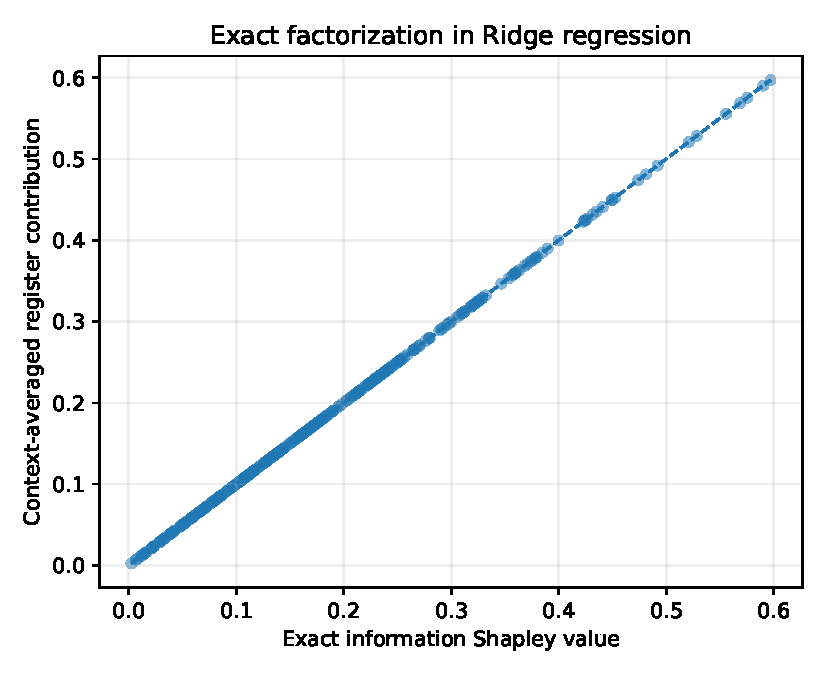
\includegraphics[width=0.68\textwidth]{assets/factorization_exact_information.pdf}
\caption{The marginal information utility obtained by refitting coincides to machine precision with $\tfrac12\log\det(I+P_S\Gamma_i)$.}
\label{fig:factorization-exact}
\end{figure}

This experiment does not replace the proof; it verifies the implementation. A second check targets the rank-one limit discussed in Equation~\eqref{eq:rankone-complete-pair}. Across the $108$ pairs in the nonlinear experiment described below, $|z|$ is reconstructed from $(\rho,\norm b)$ with maximum error $5.33\times10^{-15}$, and $\norm b$ from $(\rho,|z|)$ with maximum error $1.42\times10^{-14}$. Thus, in this scalar regime, the final two-coordinate register contains no more information than the classical leverage--studentized-innovation pair.

\subsection{Controlled non-scalar collision}
\label{subsec:experiments-nonscalar}
The collision proposition from the preceding section is turned into an experiment with no statistical noise. Two classes of rank-three registers have exactly:
\begin{itemize}
  \item the same contraction trace;
  \item the same information gain;
  \item the same Euclidean displacement norm;
  \item the same displacement norm in the post-insertion geometry;
  \item the same effect on a fixed target.
\end{itemize}
The two pairs are subjected to $400$ joint random orthogonal rotations. The target is co-rotated with the register, $t\mapsto Qt$, so the target effect remains invariant. Raw coordinates therefore carry no class information. The maximum absolute differences between the five scalarizations, computed using the full-precision constants above, are below $1.6\times10^{-15}$.

\begin{table}[H]
\centering
\caption{Classification of the two register classes after random rotations.}
\label{tab:nonscalar-collision}
\small
\begin{tabular}{@{}lc@{}}
\toprule
Representation & AUC \\
\midrule
Five matched scalar summaries & $0.500$ \\
Contraction spectrum & $1.000$ \\
Effort distribution across eigenspaces & $1.000$ \\
Complete orbit signature & $1.000$ \\
\bottomrule
\end{tabular}
\end{table}

\begin{figure}[H]
\centering
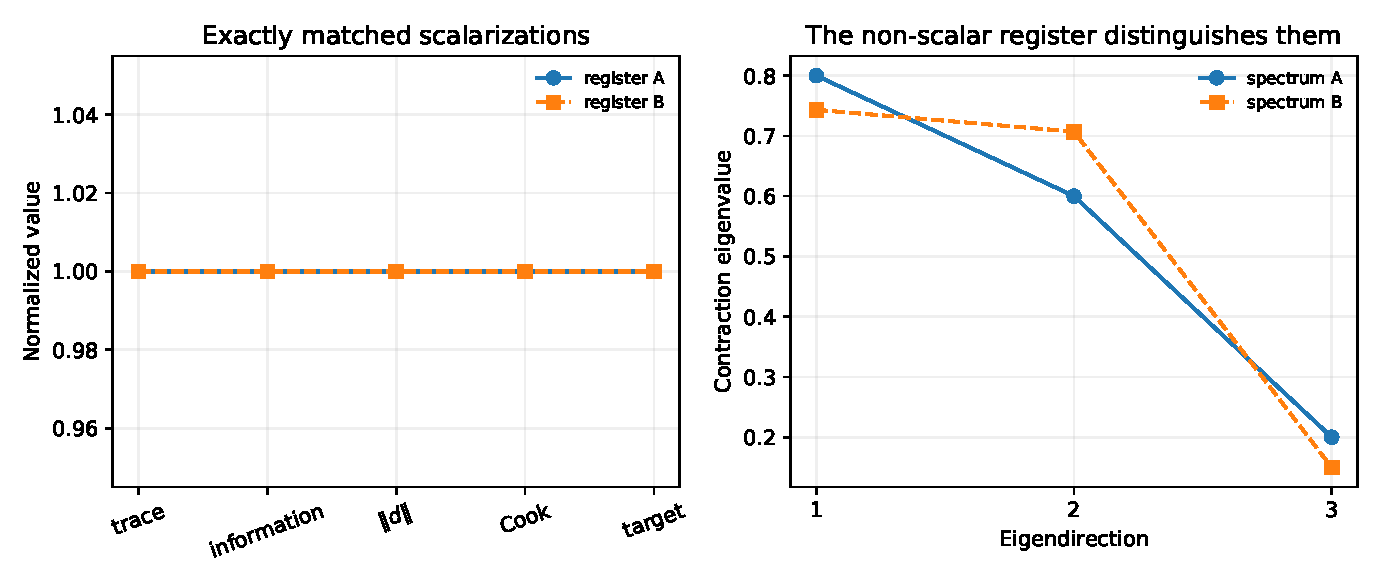
\includegraphics[width=0.80\textwidth]{assets/nonscalar_orbit_collision.pdf}
\caption{Two registers share five scalarizations but have different contraction spectra and effort distributions. Orthogonal rotations remove all coordinate-dependent information.}
\label{fig:nonscalar-collision}
\end{figure}

This experiment establishes what the scalar experiment could not: the register's own richness appears when observation rank exceeds one. It relies neither on an easily detected synthetic corruption nor on a circular selection of rare points.

\subsection{Complementarity of spectrum and energies}
The previous collision shows that five scalar summaries are insufficient, but each half of the signature still separated the two classes. We therefore add a four-mechanism factorial protocol: two contraction spectra are crossed with two effort-energy distributions. The binary label is the XOR of the two choices; by construction, spectrum alone and energies alone are each independent of the label. Four hundred joint rotations are used.

\begin{table}[H]
\centering
\caption{Complementarity of the orbit-signature components.}
\label{tab:signature-complementarity}
\small
\begin{tabular}{@{}lcc@{}}
\toprule
Representation & XOR AUC & Four-mechanism accuracy \\
\midrule
Spectrum alone & $0.500$ & $0.500$ \\
Spectral energies alone & $0.500$ & $0.500$ \\
Complete signature & $1.000$ & $1.000$ \\
\bottomrule
\end{tabular}
\end{table}

\begin{figure}[H]
\centering
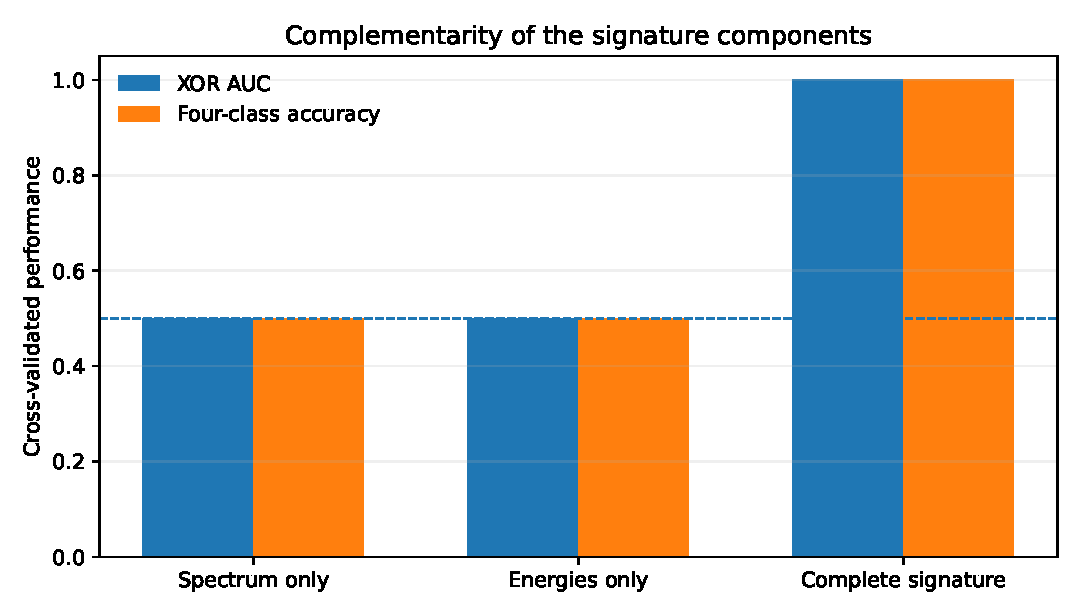
\includegraphics[width=0.72\textwidth]{assets/orbit_signature_complementarity.pdf}
\caption{Neither spectrum nor effort distribution suffices alone in the crossed protocol; their combination recovers the complete mechanism.}
\label{fig:signature-complementarity}
\end{figure}

The maximum numerical recovery error is $8.9\times10^{-16}$ for eigenvalues and $5.8\times10^{-15}$ for energies. For the binary XOR, AUC $0.5$ is chance. For four-mechanism classification, the $0.5$ accuracy of the partial representations is insufficient but above the uniform chance level $0.25$; it precisely reflects the fact that each component separates half of the classes. This control certifies complementarity of the two components of the complete invariant; it does not claim that this artificial classification is a real audit task.

\subsection{Scalar collisions in a nonlinear network}
Across six independent Friedman~\#1 datasets, a tanh network $10\to10\to1$ is trained on $500$ anchor observations. For each of $18$ base points, a label corruption and a covariate corruption are matched to produce nearly the same final tangent predictive attribution. The median relative matching error is $1.82\,\%$. All discriminative validations are grouped at the level of the independent Friedman dataset: observations from the same seed remain in the same fold using \texttt{GroupKFold}.

\begin{table}[H]
\centering
\caption{Distinguishing the corruption mechanism when final predictive attribution is matched.}
\label{tab:matched-collision}
\small
\begin{tabular}{@{}lc@{}}
\toprule
Representation & AUC \\
\midrule
Final predictive attribution, scalar & $0.499$ \\
Final functional impact, scalar & $0.442$ \\
Trajectory of scalar attribution & $0.564$ \\
Final pair $(\rho,\zeta)$ & $0.869$ \\
Trajectory of the pair & $0.879$ \\
\bottomrule
\end{tabular}
\end{table}

\begin{figure}[H]
\centering
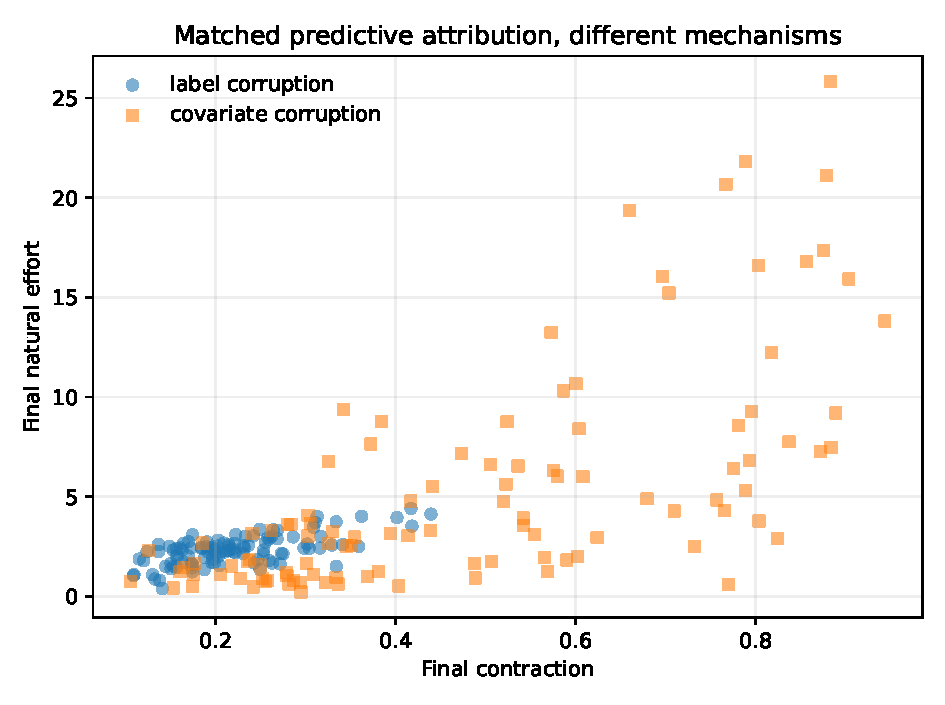
\includegraphics[width=0.72\textwidth]{assets/matched_scalar_collision_register.pdf}
\caption{Points matched to have the same final predictive attribution occupy different regions of the contraction--effort plane.}
\label{fig:matched-collision}
\end{figure}

This experiment validates the information loss induced by a single predictive attribution. It does not establish novelty relative to the classical leverage--residual pair: as shown by the rank-one equivalence, the final pair $(\rho,\zeta)$ is precisely a geometric reorganization of that classical diagnostic. Its role here is interpretive: it separates the mechanism carried by the covariates from the mechanism carried by the label.

\subsection{Functional mobility in Friedman~\#1 and frozen controls}
\label{subsec:functional-drift}
For $300$ epochs on ten independent Friedman~\#1 datasets, we train three regimes sharing the same probes: a full ReLU network $10\to8\to1$, the same frozen random feature extractor with only a linear head trained, and the fully first-order linearized model around initialization. The primary diagnostic is the functional operator $K_t^{(0)}$ and the alignment and drift quantities from Equation~\eqref{eq:alignment-drift}.

\begin{table}[H]
\centering
\caption{Functional mobility and performance between initialization and epoch 300.}
\label{tab:functional-drift}
\small
\begin{tabular}{@{}lccc@{}}
\toprule
Regime & Alignment of $K^{(0)}$ & Normalized drift & Test MSE \\
\midrule
Full network & $0.815\pm0.036$ & $0.606\pm0.058$ & $0.1020\pm0.0090$ \\
Frozen feature extractor & $1.000$ & $0.000$ & $0.6502\pm0.1243$ \\
Linearized model & $1.000$ & $0.000$ & $0.2917\pm0.0224$ \\
\bottomrule
\end{tabular}
\end{table}

\begin{figure}[H]
\centering
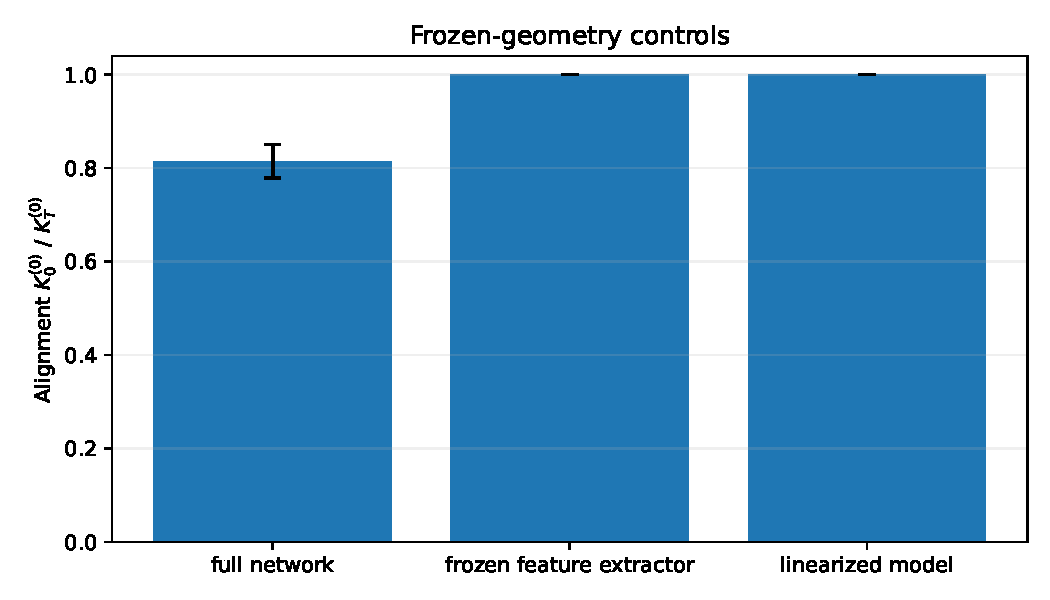
\includegraphics[width=0.80\textwidth]{assets/functional_drift_controls.pdf}
\caption{The full network changes the functional operator; both frozen-geometry controls preserve $K_0^{(0)}$ exactly.}
\label{fig:functional-drift}
\end{figure}

The three rows do not live in exactly the same tangent space. For the \emph{frozen feature extractor}, the declared parametric subspace is that of the trainable linear head alone; in this reduced space, its head Jacobian, and therefore $K_t^{(0)}$, is constant by construction. If the frozen extractor parameters were formally retained in the full tangent space, the total Jacobian could depend on the head weights. The \emph{linearized model} control, by contrast, uses the same number of parameter coordinates as the full network but fixes the Jacobian at initialization: it is the lazy control in the same ambient space.

The decrease in alignment of the full network, absent from these explicitly frozen controls, establishes only that its functional operator is not constant in this protocol. It does not prove that this mobility alone causes the MSE gap between regimes. A second computation, restricted to the full network, gives hidden-representation Gram alignment $0.574\pm0.056$, initial--final rank correlation of contractions $0.834\pm0.023$, and median relative drift of raw Jacobians $2.509\pm0.441$. These are auxiliary diagnostics: the hidden Gram depends on the chosen representation and raw Jacobian drift depends on parameterization. The operator-level control $K_t^{(0)}$ carries the main conclusion.

At the final epoch, register medians separate the controlled contaminations:
\begin{table}[H]
\centering
\caption{Final qualification of the probes in Friedman~\#1.}
\label{tab:nonlinear-groups}
\small
\begin{tabular}{@{}lcc@{}}
\toprule
Group & Median contraction & Median natural effort \\
\midrule
Ordinary clean & $0.166$ & $0.386$ \\
Rare clean & $0.221$ & $0.541$ \\
Label outlier & $0.159$ & $7.636$ \\
Covariate outlier & $0.751$ & $15.844$ \\
Mixed contamination & $0.746$ & $28.638$ \\
\bottomrule
\end{tabular}
\end{table}
Label corruption leaves contraction nearly ordinary and increases effort. Covariate corruption strongly increases contraction; in this network, it also increases effort because the prediction is displaced. The register therefore does not promise perfect causal separation, but a decomposition of the channels through which the point acts.

\subsection{The history of an observation is not its final state}
In a stagewise experiment, $400$ identically distributed observations are randomly assigned to an early- or late-exposure group. The network is trained successively on the first group, on the second, and then on the union. Eight independent datasets are used.

\begin{table}[H]
\centering
\caption{AUC for recovering exposure order after a common final phase.}
\label{tab:stagewise}
\small
\begin{tabular}{@{}lcc@{}}
\toprule
Representation & Mean AUC & Standard deviation \\
\midrule
Final predictive attribution & $0.491$ & $0.035$ \\
Final pair $(\rho,\zeta)$ & $0.494$ & $0.026$ \\
Predictive-attribution trajectory & $0.639$ & $0.020$ \\
Residual trajectory & $0.726$ & $0.025$ \\
Register trajectory & $0.727$ & $0.023$ \\
\bottomrule
\end{tabular}
\end{table}

\begin{figure}[H]
\centering
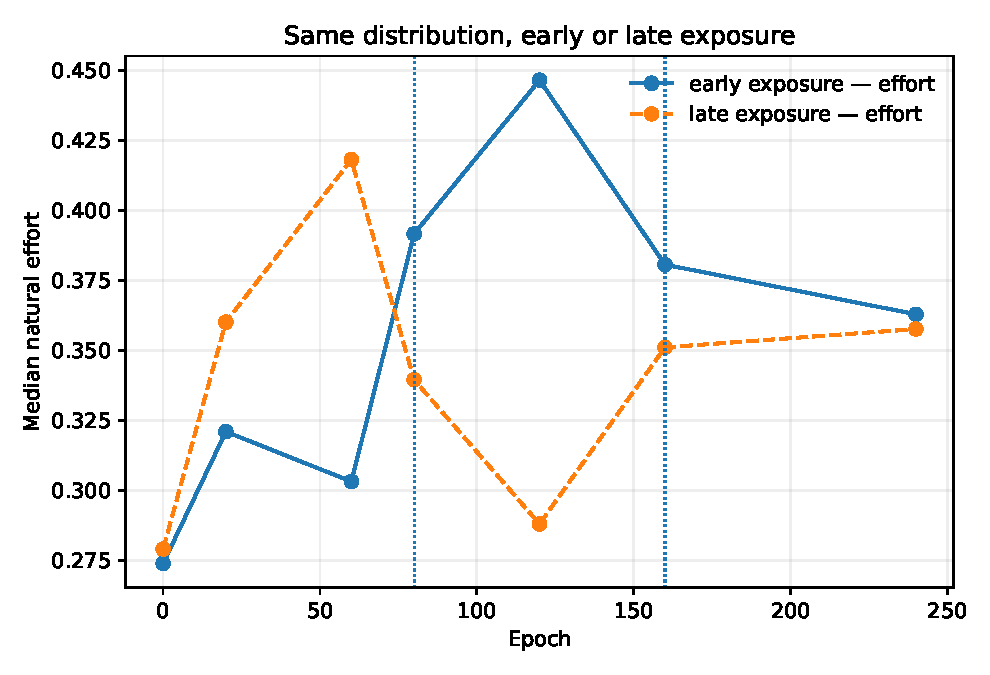
\includegraphics[width=0.76\textwidth]{assets/stagewise_dynamic_register.pdf}
\caption{The common phase brings final states closer, whereas the trajectories retain the exposure order.}
\label{fig:stagewise}
\end{figure}

The result supports the need for temporal accounting, but not a general superiority of the dynamic register: the residual trajectory reaches almost the same AUC. Here the register provides a decomposition of the phenomenon, not an established discriminative gain.

\subsection{California Housing: controlled local qualification}
\label{subsec:california}
California Housing is used with linear Ridge regression and label corruptions injected into $5\,\%$ of the training set. Rare but clean points and controlled duplications are added to test false positives. At fixed $\lambda$, the global score is the studentized deleted residual obtained through the hat-matrix identity, without retraining $n$ models. A point is excluded from its own neighborhood. Neighborhood, local-shrinkage, and $\lambda$ parameters are selected on a clean validation set; the final test remains hidden. This is algebraic leave-one-out with self-excluded neighborhoods, not $K$-fold cross-fitting.

\begin{table}[H]
\centering
\caption{Detection of corrupted labels: global score, Euclidean neighborhood, and Ridge-geometric neighborhood.}
\label{tab:california}
\scriptsize
\begin{tabular}{@{}lcccc@{}}
\toprule
Amplitude & Score & AUC & Precision at top-$k$ & Rare clean points at top-$k$ \\
\midrule
$0.75\sigma$ & global & $0.810$ & $0.173$ & $9.82\,\%$ \\
                & local Euclidean & $0.858$ & $0.319$ & $4.60\,\%$ \\
                & local geometric & $0.864$ & $0.350$ & $4.43\,\%$ \\
$1.5\sigma$  & global & $0.950$ & $0.480$ & $5.73\,\%$ \\
                & local Euclidean & $0.959$ & $0.618$ & $2.61\,\%$ \\
                & local geometric & $0.959$ & $0.636$ & $2.36\,\%$ \\
$3\sigma$      & global & $0.997$ & $0.914$ & $1.61\,\%$ \\
                & local Euclidean & $0.996$ & $0.868$ & $1.02\,\%$ \\
                & local geometric & $0.995$ & $0.870$ & $0.98\,\%$ \\
\bottomrule
\end{tabular}
\end{table}

\begin{figure}[H]
\centering
\begin{subfigure}[t]{0.48\textwidth}
\centering
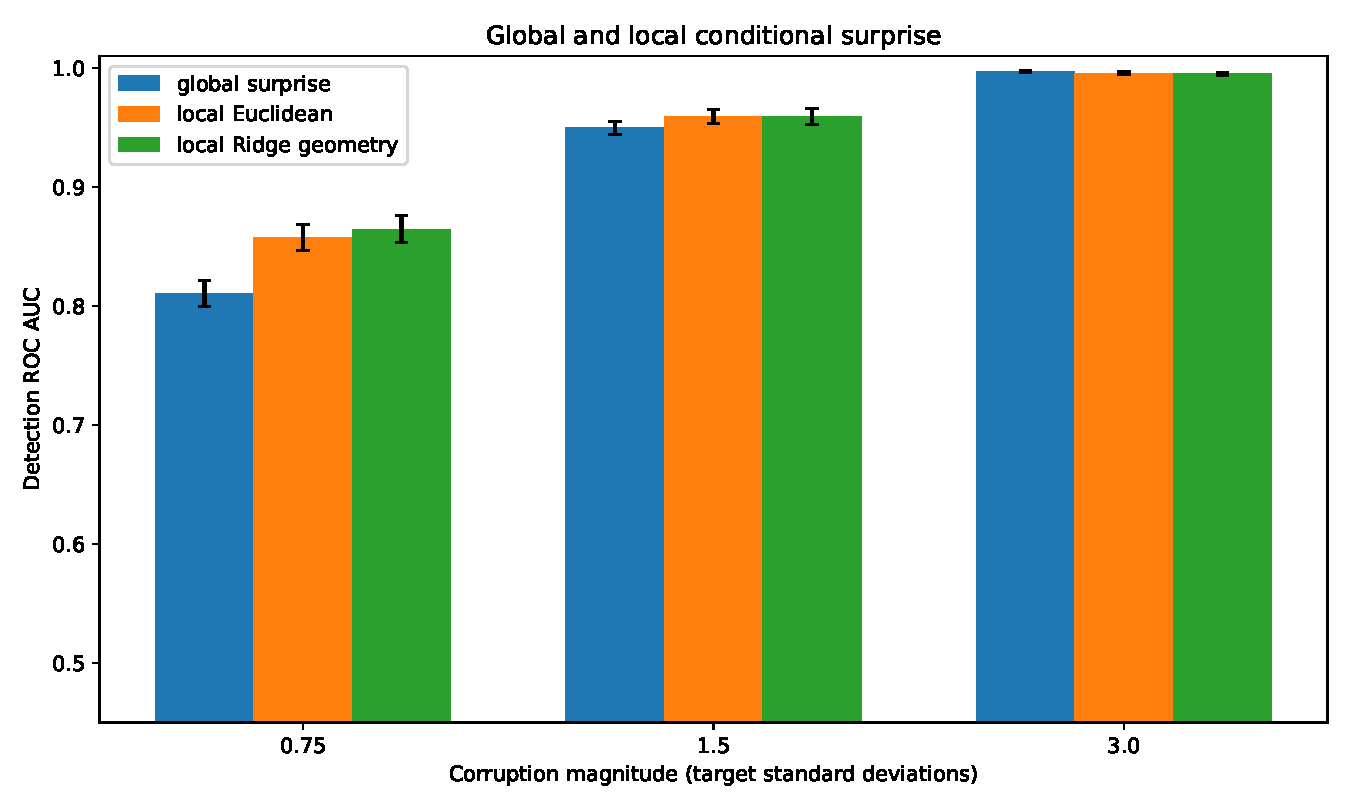
\includegraphics[width=\linewidth]{assets/california_auc.pdf}
\caption{Detection AUC.}
\end{subfigure}\hfill
\begin{subfigure}[t]{0.48\textwidth}
\centering
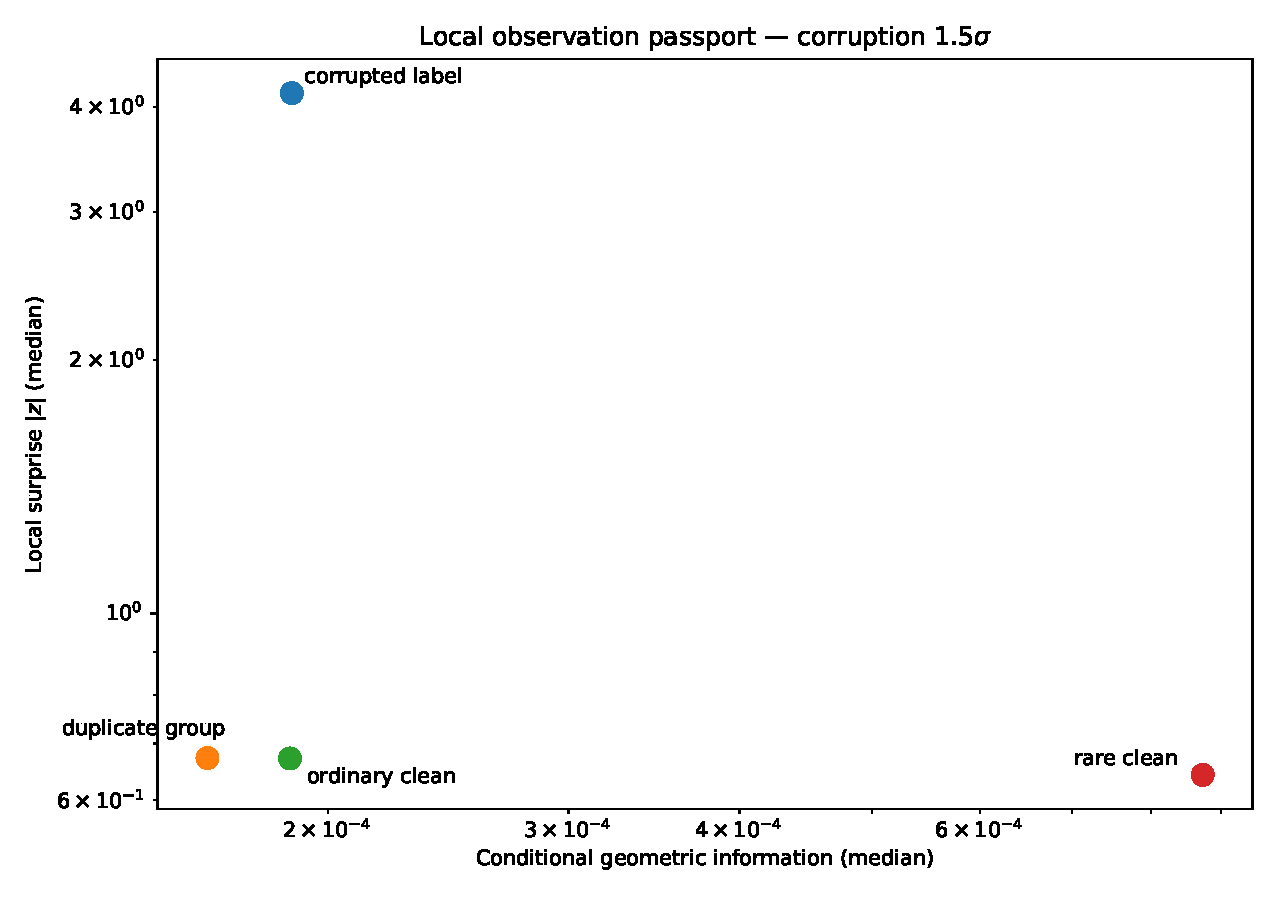
\includegraphics[width=\linewidth]{assets/california_passport.pdf}
\caption{Contribution--surprise passport.}
\end{subfigure}
\caption{Local correction helps mainly when corruption is weak and confounded with misspecification of the global model.}
\label{fig:california}
\end{figure}

The local correction substantially improves the top of the ranking for weak and moderate corruptions while protecting rare clean points. Most of the gain comes from local contextualization; at $0.75\sigma$, the Ridge geometry adds about $0.007$ AUC and $0.031$ top-$k$ precision over the Euclidean neighborhood. For gross corruptions, the global residual is already nearly perfect. Finally, directly using these scores as loss weights worsens test MSE: an audit passport is not automatically an optimal regression coefficient.

\subsection{SeLoger: robustness on raw data}
\label{subsec:seloger}
The SeLoger file contains $8{,}899$ raw rows and $3{,}815$ listing identifiers. No structural cleaning, deduplication, or removal of atypical prices is applied to the training set. The target is log price; internal splits are performed by identifier. Synthetic contaminations are injected into non-duplicated listings so that the main result is not a deduplication effect.

\paragraph{Internal holdout and representative rule.}
Before the calibration specific to this version, identifiers are split once and for all into two globally disjoint sets:
\[
\mathcal D_{\rm dev}\cap\mathcal D_{\rm eval}=\varnothing,
\qquad
|\mathcal D_{\rm dev}|=763,
\qquad
|\mathcal D_{\rm eval}|=3{,}052.
\]
All robust thresholds are selected only within $\mathcal D_{\rm dev}$; the ten final splits are performed exclusively within $\mathcal D_{\rm eval}$. This pool is an \emph{internal holdout newly isolated for versions 6--7}, not a historically blind external test: earlier exploratory versions had already used the same corpus. SHA--256 hashes of both identifier lists are included in the archive.

The training set retains every row. Validation and test use a deterministic representative for each listing: the median for numerical columns and the first modal value under lexicographic ordering for non-numerical columns. Among the $64$ repeated groups, $21$ are not perfectly identical, amounting to $0.55\,\%$ of the listings; only the columns \texttt{number} and \texttt{position} vary within these groups. This aggregation replaces the former first-row rule and removes dependence on file order.

\paragraph{Estimators actually tested.}
In the main stress test, masses and the semantic gate are deliberately disabled:
\[
\boxed{\pi_i=\chi_i=1.}
\]
The experiment isolates only the budgets $a_i^X$ and $a_i^Y$. The implementation adds a constant coordinate to the design and uses \texttt{fit\_intercept=False}; the intercept is therefore penalized. BGR and the Schweppe-type baseline call the same fitting functions during calibration and evaluation, with at most twelve IRLS iterations and relative tolerance $2\times10^{-5}$.

For each family, the selection rule is
\[
\frac13\sum_{s=1}^{3}
\frac{\mathrm{RMSE}_{s,\rm robust}}
     {\mathrm{RMSE}_{s,\rm Ridge}}
\le 1.005,
\]
after which the most aggressive admissible pair is retained. Both families independently select $q_X=0.90$ and $\kappa_Y=2$. For BGR, the mean ratio is $0.98747$ and the maximum ratio $1.00230$; for the Schweppe-type baseline, they are $0.98716$ and $1.00110$. This selection is conditional on the nominal internal holdout, not a universal non-inferiority guarantee.

The baseline called \emph{Huber with geometric scale} below does not use geometric weights in its final regression, but its residual scale is estimated after a preliminary fit weighted by $a_i^X$. A separate ablation, reported below, adds a pure Huber estimator whose scale comes from ordinary Ridge.

Two evaluation domains are reported:
\[
\mathrm{RMSE}_{\rm all}
\quad\text{over all distinct listings,}
\]
and
\[
\mathrm{RMSE}_{\rm plausible}
\quad\text{after excluding, at test time only, }
\text{area}\le0,\ \text{rooms}>20,\ \text{bedrooms}>10.
\]
The second domain isolates learning robustness without making the primary metric depend on manifestly out-of-domain covariates; the first preserves transparency about this convention.

\begin{table}[H]
\centering
\caption{Nominal performance on the internal SeLoger holdout. Mean $\pm$ standard deviation over ten overlapping splits, per distinct listing.}
\label{tab:seloger-nominal}
\small
\begin{tabular}{@{}lcc@{}}
\toprule
Method & $\mathrm{RMSE}_{\rm all}$ & $\mathrm{RMSE}_{\rm plausible}$ \\
\midrule
Ridge & $0.25838\pm0.01407$ & $0.25816\pm0.01412$ \\
Huber (geometric scale) & $0.25960\pm0.01446$ & $0.25935\pm0.01448$ \\
Geometry only & $0.25810\pm0.01447$ & $0.25807\pm0.01449$ \\
Schweppe-type & $0.25964\pm0.01467$ & $0.25945\pm0.01470$ \\
BGR & $0.25944\pm0.01481$ & $0.25938\pm0.01483$ \\
\bottomrule
\end{tabular}
\end{table}

The mean nominal cost of BGR relative to Ridge is $0.001220$ in plausible RMSE, or $0.47\,\%$. The ten splitwise differences give the descriptive interval
\[
[-0.00031,\ 0.00275]
\]
around the mean; BGR is better on five splits and worse on five. No conventional $p$-value is reported because training and test sets overlap across repetitions.

\begin{table}[H]
\centering
\caption{Increase in plausible/all-listing RMSE relative to each method's clean nominal state, under $5\,\%$ contamination.}
\label{tab:seloger-ablation}
\scriptsize
\setlength{\tabcolsep}{4.5pt}
\begin{tabular}{@{}lccccc@{}}
\toprule
Scenario & Ridge & Geom. Huber & Geometry & Schweppe-type & BGR \\
\midrule
Label, amplitude $4$
& $0.05745/0.05914$
& $0.00115/0.00132$
& $0.05881/0.06167$
& $\mathbf{0.00113}/0.00132$
& $0.00114/0.00138$ \\
Covariates, amplitude $50$
& $0.14523/0.14495$
& $0.11776/0.11746$
& $0.01463/0.02033$
& $0.00126/0.00167$
& $\mathbf{-0.00006/-0.00001}$ \\
Mixed, amplitudes $50$ and $4$
& $0.18145/0.18143$
& $0.07702/0.07725$
& $0.01506/0.02000$
& $0.00313/0.00407$
& $\mathbf{0.00010/0.00018}$ \\
Diffuse Gaussian noise, $\sigma=0.4$
& $\mathbf{0.02416}/0.02428$
& $0.02730/0.02712$
& $0.02410/0.02438$
& $0.02737/0.02719$
& $0.02727/0.02732$ \\
\bottomrule
\end{tabular}
\end{table}

Under vertical outliers, the three estimators with bounded residual score achieve similar protection. Under high leverage, geometric clipping sharply reduces degradation, the Schweppe-type estimator lowers it to $0.00126$, and BGR's degradation is numerically indistinguishable from zero. Under mixed contamination, the plausible degradation of BGR is $0.00010$, compared with $0.00313$ for Schweppe-type, $0.01506$ for the geometric gate alone, and $0.18145$ for Ridge. Under diffuse Gaussian noise, Ridge and the geometric gate alone remain better in this protocol.

The cellwise scenario reproducing $\mathrm{area}=0$, $53$ rooms, or $22$ bedrooms yields plausible degradations of $0.00222$ for Ridge, $0.00031$ for Huber, and $0.00090$ for BGR. These values do not turn norm clipping into a semantic detector: an impossible covariate of moderate norm still requires a validity gate $\chi_i$ or a cellwise robust method.

\begin{figure}[H]
\centering
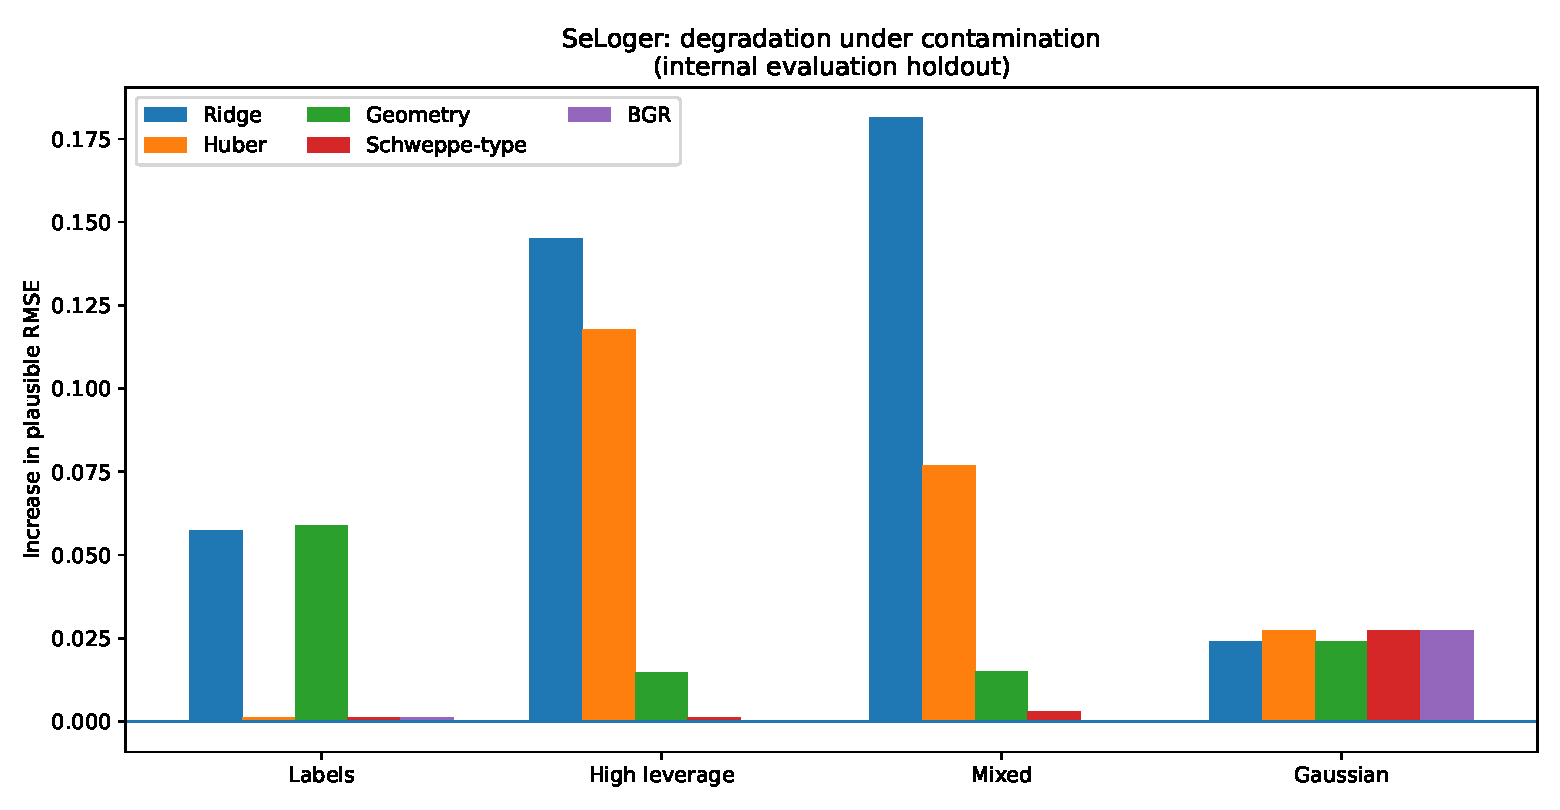
\includegraphics[width=0.94\textwidth]{assets/seloger_bgr_core_scenarios.pdf}
\caption{Degradation of plausible RMSE in the main internal-holdout scenarios. Bars compare methods relative to their own nominal performance.}
\label{fig:seloger-bgr}
\end{figure}

\paragraph{Ablations requested by the review.}
Across five splits of the evaluation pool, a pure Huber estimator, calibrated separately with a scale obtained from ordinary Ridge, selects $\kappa_Y=1.5$. Its degradation under vertical contamination is $0.00075$, compared with $0.00102$ for the geometrically stabilized-scale baseline. Their nominal RMSEs are respectively $0.26607$ and $0.26507$. The ablation conclusion therefore does not depend on geometric pre-fitting: a bounded residual score is sufficient for vertical contamination, but the two scale choices are not identical.

The geometric threshold at quantile $q_X=0.90$ is on average $3.6765$ when computed over raw rows, compared with $3.2735$ using one median representative per identifier or quantile weights $1/m_g$. Despite this difference of about $12\,\%$, BGR degradations remain near zero under the gross stress test: for leverage, $-0.00015$, $-0.00011$, and $-0.00011$; for mixed contamination, $-0.00006$, $-0.00001$, and $-0.00001$. This five-split sensitivity analysis shows that calibration of $\kappa_X$ does depend on the notion of mass, while the qualitative conclusion of the extreme stress test remains stable.

The ablation supports the contraction--displacement interpretation: the innovation gate protects against label outliers, the geometric gate protects against high-leverage covariates, and their combination is necessary for mixed contamination. BGR remains a regularized Mallows-type GM-estimator; the experiment validates a mechanism in this protocol, not algorithmic novelty or general dominance over the best robust estimators.

\subsection{Concrete Compressive Strength: public stress test}
To make the mechanism verifiable without the private SeLoger file, we reproduce the same type of stress test on Concrete Compressive Strength, a UCI dataset with $1{,}030$ observations, eight numerical variables, and compressive strength in MPa as target \citep{yeh1998concrete}. Recipes with exactly identical covariates are grouped before any split. A global development pool containing $25\,\%$ of the groups is used for calibration over five splits; the ten evaluation splits are performed on the remaining groups. Here, the residual scales of all methods come from ordinary Ridge.

The development constraint is stricter than for SeLoger: mean nominal ratio below $1.005$ and maximum ratio below $1.01$. It selects $q_X=0.99$ and $\kappa_Y=4$ for BGR. On the evaluation pool, this calibration does not transfer perfectly: nominal BGR RMSE is $0.63432$, compared with $0.62183$ for Ridge, a cost of about $2.0\,\%$. This cost is retained because it prevents presenting the robust result without its nominal trade-off.

\begin{table}[H]
\centering
\caption{Public Concrete experiment: nominal RMSE and RMSE increase under $5\,\%$ contamination. Standardized target; ten overlapping splits of the evaluation pool.}
\label{tab:concrete-public}
\scriptsize
\begin{tabular}{@{}lrrrr@{}}
\toprule
Method & Nominal & Labels $A=4$ & Leverage $A=50$ & Mixed \\
\midrule
Ridge & $0.62183$ & $0.01086$ & $0.34651$ & $0.34750$ \\
Pure Huber & $0.63340$ & $\mathbf{0.00146}$ & $0.31401$ & $0.26987$ \\
Geometry only & $0.63199$ & $0.01195$ & $0.11931$ & $0.11557$ \\
Schweppe-type & $0.66268$ & $-0.00055$ & $0.03649$ & $0.03478$ \\
BGR & $0.63432$ & $0.00414$ & $\mathbf{0.02541}$ & $\mathbf{0.02416}$ \\
\bottomrule
\end{tabular}
\end{table}

The public dataset recovers the separation of mechanisms: Huber mainly reduces vertical outliers, whereas methods with a geometric gate resist leverage. BGR achieves the smallest degradation under leverage and mixed contamination among the retained configurations, but it dominates neither Huber on labels nor Ridge nominally. Differences under diffuse Gaussian noise are small and vary in sign; they are not used as an argument of superiority.

\begin{figure}[H]
\centering
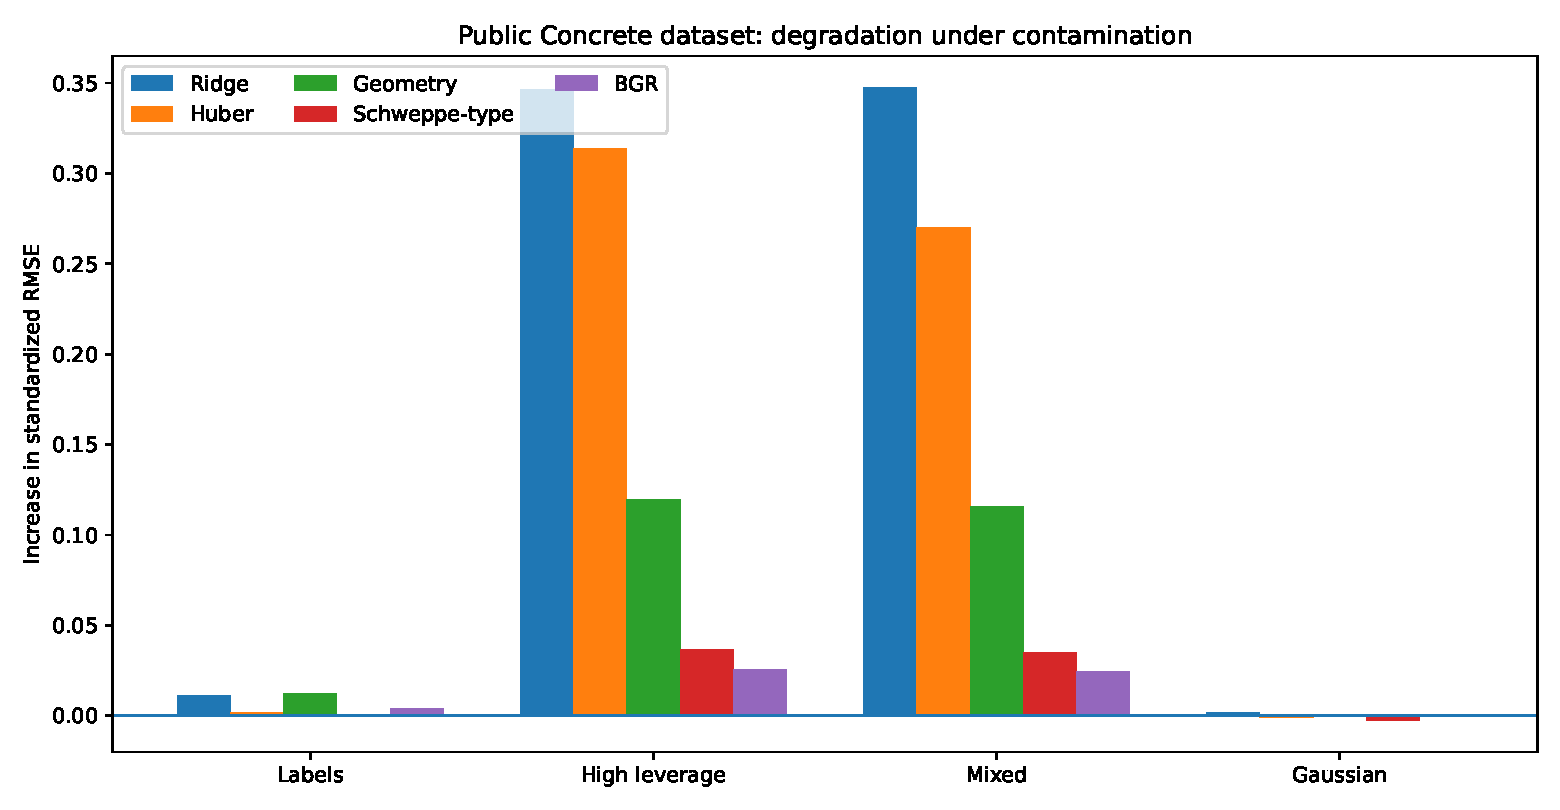
\includegraphics[width=0.88\textwidth]{assets/concrete_bgr_public_stress.pdf}
\caption{Public Concrete experiment: increase in RMSE relative to each method's own nominal state. The distinct nominal cost of each estimator must be read together with Table~\ref{tab:concrete-public}.}
\label{fig:concrete-public}
\end{figure}

This public replication strengthens validation of the mechanism while also showing its limitation: satisfying a nominal constraint on development does not guarantee the same cost on another pool. It therefore supports a conditional robustness interpretation, not universal dominance of BGR.

\subsection{What the experiments do and do not establish}
The experimental results support five conclusions:
\begin{enumerate}
  \item the static factorizations are exact when their assumptions hold;
  \item non-scalar structure becomes possible as soon as rank exceeds one, and a simultaneous collision of five scalarizations is explicitly established in rank three;
  \item the functional register genuinely evolves in the nonlinear protocol;
  \item the contraction--innovation decomposition provides a coherent architecture for auditing and for distinct robust budgets;
  \item the SeLoger and Concrete controls reproduce this separation under gross contamination while revealing nominal costs, calibration effects, and the absence of dominance under diffuse noise.
\end{enumerate}
They do not establish:
\begin{itemize}
  \item general superiority over Data Shapley, TRAK, or influence functions for every utility;
  \item novelty of the leverage--residual pair in scalar regression;
  \item a universal predictive gain of the BGR prototype or cost-free calibration transfer;
  \item automatic detection of semantic covariate errors;
  \item a global guarantee for nonconvex networks.
\end{itemize}

% -----------------------------------------------------------------------------
\section{Prior Work and Positioning}
\label{sec:related-work}
% -----------------------------------------------------------------------------
\subsection{Spectral theory, orthogonal invariants, and jet bundles}
The classification of the pair $(B,b)$ is not new as an abstract result. It follows from the spectral decomposition of a self-adjoint operator and the action of its orthogonal stabilizer on a distinguished vector. Spectral multiplicity theory, orthogonal matrix invariants, and vector invariants provide the classical framework \citep{halmos1951,weyl1946,sibirskii1967,sibirskii1968,khadzhiev1967}. Our contribution lies in selecting the conditional datum $(G_S,\Gamma_i,\alpha_i)$, interpreting its signature as an observation register, and explicitly factoring learning diagnostics through it. Likewise, the term ``jet'' is reserved for its standard meaning \citep{saunders1989}: the object studied here is a relative Gauss--Newton quadratic datum decorated by the context.

\subsection{Local influence, diagnostics, and robustness}
Leverage, studentized residuals, and Cook's distance belong to the tradition of regression diagnostics \citep{cook1977}. Differential geometry of perturbations and local influence was already developed by \citet{cook1986}, then connected to leverage and curvature in nonlinear regression by \citet{stlaurent1993}. Influence functions and infinitesimal robustness go back in particular to \citet{hampel1974}; Huber and bounded-influence regression estimators limit extreme residuals and leverage points \citep{huber1964,mallows1975,krasker1982,richardson1997}. The Versatile Influence Function now extends this analysis to non-decomposable objectives such as contrastive, ranking, or graph losses \citep{deng2025vif}; our current construction instead assumes an explicit decomposition into contributions of observations or declared blocks. Cellwise robust M-regression also addresses contaminated cells, a problem that norm clipping does not solve \citep{filzmoser2020}.

This paper therefore claims neither the leverage--residual combination nor the principle of bounded influence. Mallows and Schweppe forms belong to this tradition of GM-estimators \citep{mallows1975,richardson1997,maronna2006robust}. The candidate contribution is the orbit classification of the local triplet $(G,\Gamma,\alpha)$ and the simultaneous preservation of the observability operator and the effort before scalarization.

\subsection{Scores, Fisher geometry, tangent kernels, and representations}
The Fisher kernel of \citet{jaakkola1998} already constructs a similarity from cotangent scores in an information metric. Natural gradient and its parameterization-invariant geometries are prior work \citep{amari1998,ollivier2015,martens2020}; the relation between online natural gradient and the Kalman filter is made explicit by \citet{ollivier2017}. Degenerate pullback metrics, pseudometrics, and associated quotients for networks are studied directly by \citet{benfenati2023singular}; this prior work in particular delimits our main assumption $G_S\succ0$ and quotient-based extensions. NTK and GTK describe functional operators derived from the Jacobian and a parametric cometric \citep{jacot2018,bai2025gtk}. Evolution and alignment of tangent features are also studied by \citet{baratin2021}.

The register is therefore not the first geometric object built from scores or Jacobians. It differs through its conditioning on a single observation and through jointly retaining the positive second-order term $\Gamma_i$ and the first-order term $\alpha_i$, classified relative to the collective geometry.

\subsection{Data valuation and semivalues}
Data Shapley chooses a utility and averages marginal contributions over contexts \citep{ghorbani2019}. Beta--Shapley and Data Banzhaf modify the context distribution or the stability of this average \citep{kwon2022,wang2023banzhaf}. Volume-based methods explicitly address robustness to replication \citep{xu2021volume}; a recent preprint proposes geometric valuation by leverage and ridge leverage \citep{mendozasmith2025}. Datamodels and TRAK develop other approximations of the effect of data on predictions \citep{ilyas2022,park2023trak}.

Three works from 2026 further tighten this neighborhood. The Bayesian information approach of \citet{tailor2026bayesian} measures predictive information loss induced by data removal and approximates it using tangent features. Eigen-Value \citep{choi2026eigenvalue} values points through perturbations of covariance-eigenvalue ratios under domain shift. Finally, Symbolic Mechanistic Data Attribution \citep{habibi2026smda} fits Ridge regression on interpretable features and analytically decomposes data effects into an activation-mediated path and an output-mediated path. These works confirm that information, spectra, tangent features, and input--output separation are already active directions. Our result remains narrower: it jointly classifies the positive operator $B$ and the effort $b$, relative to context, before any scalar utility is selected.

The paper does not claim that Shapley must be scalar in principle: vector-valued utilities may be defined. Common uses of Data Shapley nevertheless choose a scalar utility before averaging and do not automatically retain the mixed tensorial structure $(\Gamma_i,\alpha_i)$. Our exact result is narrower: for additive information utility, the marginal contribution is a scalarization of the register; for a smooth predictive utility, the local effect or finite path provides the contribution before contextual averaging.

\subsection{Dynamic attribution}
Integrating a sensitivity along a participation path has direct precedent in dynamic valuation methods, notably NDDV \citep{liang2024nddv}. The Memory--Perturbation Equation likewise relates model memory during training to sensitivity under data perturbations and unifies several existing measures \citep{nickl2023mpe}. In its current formulation, NDDV connects finite marginal contribution to an integral of sensitivities along a state dynamics and discusses its relation to Shapley, Banzhaf, and leave-one-out. Our path theorem is an application of the implicit-function theorem and is not, in isolation, a deep novelty. The proposed distinction is that the path of minima is equipped at every instant with an observability--effort decomposition and a contraction operator. This distinction should be compared more directly with state--adjoint formulations and the MPE in future work.

\subsection{Boundary of the contribution}
\begin{statementbox}{Defensible claim}
The central result is neither a new robust estimator nor a new semivalue. It is the complete characterization, up to local reparameterization, of the relative quadratic model of an observation by the orbit signature of $(B,b)$, together with a proof that several common diagnostics are non-injective projections of this object. The path register extends this accounting to the case in which geometry and model evolve.
\end{statementbox}
Absolute bibliographic priority for a register with exactly this combination cannot be established from the search conducted here alone. The paper claims a theorem and a precise organization, not the general invention of geometric influence, dynamic valuation, or robustness.

% -----------------------------------------------------------------------------
\section{Limitations and Open Questions}
% -----------------------------------------------------------------------------
\begin{enumerate}
  \item \textbf{Locality.} The orbit theorem concerns a local quadratic model and a positive geometry. An indefinite exact Hessian would require classification under a different group and does not directly inherit the same contraction interpretations. The relative quadratic datum also retains neither the loss constant nor output-error components lying in $\Ker J_i^*$. It now explicitly distinguishes this parametric kernel from the output-curvature kernel $\Ker(W_i h_i^\sharp)$.
  \item \textbf{Degeneracy.} We assume $G_S\succ0$. Generic low-rank strata of $B$ are classified here, but repeated positive eigenvalues, zero spectral energies, rank changes along a trajectory, and the case in which the collective geometry $G_S$ itself is singular still require a stratified theory or passage to an identifiable quotient.
  \item \textbf{Path of minima.} Nonlinear insertion assumes a regular branch of local minima. Bifurcations, basin changes, or singular Hessians may interrupt the path.
  \item \textbf{Background metric.} The functional operator $K_t^{(0)}$ depends on the declared choice of $g_0$. Reparameterization invariance does not remove this substantive choice.
  \item \textbf{Multiple configurations.} Individual signatures do not contain the mutual angles among several prospective observations; joint selection or auditing requires simultaneous invariants in a common frame.
  \item \textbf{Qualification versus weighting.} An informative, discordant, or influential point is not necessarily bad. The experiments show that good qualification does not automatically yield an optimal loss weight.
  \item \textbf{Semantic validity.} A constraint such as ``strictly positive area'' does not follow from differential geometry alone. It requires a domain, a conditional model, or subject-matter knowledge.
  \item \textbf{Experimental comparisons.} Controlled corruptions isolate mechanisms but do not replace natural annotations. The added Schweppe-type baseline shares the same leverage proxy as BGR, although its thresholds are calibrated separately under the same nominal constraint; a complete comparison should still include Cook, robust leverage, influence functions, TRAK, semivalues, high-breakdown-initialized Krasker--Welsch, and cellwise methods across several independent tasks.
  \item \textbf{Scalability.} Full spectra and metric inverses are expensive in large networks. Low-rank approximations, matrix--vector products, and randomized sketches remain to be developed.
\end{enumerate}

% -----------------------------------------------------------------------------
\section{Conclusion}
% -----------------------------------------------------------------------------
A training observation cannot be reduced to a weight. Locally, it has a first-order component, the cotangent effort $\alpha_i$, and a positive second-order component, the observability tensor $\Gamma_i$, both relative to the collective geometry $G_S$. The triplet $(G_S,\Gamma_i,\alpha_i)$ is complete for the parametric action of the declared Gauss--Newton quadratic model, up to an additive constant, once the loss, output metric, collective geometry, and background metric have been fixed. An absolute utility may be completed by $c_i=\ell_i(\widehat\theta_S)$. On the principal stratum, the quotient has $2p$ global coordinates. More generally, an observation of rank $r<p$ belongs to a generic stratum of dimension $2r+1$, reduced to $2r$ when $b\in\Img B$. The compatibility lemma shows that the latter situation is natural for a quadratic loss with non-degenerate output curvature; the scalar case is therefore exactly the compatible $r=1$ stratum.

After whitening, this generator becomes a pair $(B,b)$ defined up to orthogonal action. The classification theorem shows that its orbit is fully determined by the spectrum of $B$ and the energy of $b$ in each eigenspace. Every reparameterization-invariant local quadratic quantity therefore factors through this signature. Leverage, information gain, Cook's distance, influence, and several marginal contributions appear as projections of this object.

The scalar limit is essential: when the observation is rank one, the invariant register reduces, for $q_i>0$, to the leverage--studentized-innovation-magnitude pair; the sign and invisible output components must be retained separately. Non-scalar structure becomes possible as soon as rank exceeds one; our simultaneous collision of five scalarizations is constructed in rank three and shows that these identical summaries are insufficient to recover the signature.

In the nonlinear setting, exact response depends on the Hessian whereas observability qualification relies on Gauss--Newton. Finite insertion follows a reweighting path and produces geometric feedback because the displacement changes the Jacobians and output metrics. Tracking $K_t^{(0)}$ and the representations confirms this mobility in the Friedman experiment without conflating raw parametric drift with functional change.

The same framework finally clarifies why label outliers, high-leverage points, invalid cells, and collection dependence call for different mechanisms. Displacement budgets, contraction budgets, structural validity, and statistical mass are distinct coordinates. The tabular prototypes illustrate this separation, but their nominal costs and calibration sensitivity confirm that they are not the central contribution of the paper; they belong to the tradition of GM-estimators.

The proposed contribution is therefore a local, conditional theory for qualifying observations before scalarization:
\[
\boxed{
\text{collective geometry}
+\text{point observability}
+\text{label effort}
=\text{contribution signature}.
}
\]
Its scientific scope does not lie in a universal victory over Ridge or Shapley, but in an intrinsic characterization of the information lost when this signature is replaced by a single score.

% -----------------------------------------------------------------------------
\appendix
\section{Supplementary Proofs}
\label{app:proofs}
\subsection{Weighted pseudoinverse and the Tikhonov limit}
\label{app:pseudoinverse}
Let $R\succ0$, $M\succ0$, and
\[
B=R^{-1/2}AM^{-1/2},
\qquad
z=R^{-1/2}(y-A\theta_0).
\]
Setting $u=M^{1/2}(\theta-\theta_0)$, the least-squares problem becomes $\min_u\norm{Bu-z}^2$. Its minimizers are $B^\dagger z+\Ker B$, and the one of minimum norm is $B^\dagger z$. Hence
\[
\theta_M^\dagger=\theta_0+M^{-1/2}B^\dagger z,
\]
with $\theta_M^\dagger-\theta_0\perp_M\Ker A$. If $B=U\Sigma V^\top$, the Tikhonov minimizer is
\[
\theta_\lambda-\theta_0
=M^{-1/2}\sum_j\frac{\sigma_j}{\sigma_j^2+\lambda}\inner{z}{u_j}v_j.
\]
Every coefficient converges to $1/\sigma_j$ when $\sigma_j>0$ and to $0$ when $\sigma_j=0$, giving the weighted Moore--Penrose limit.

\subsection{Details of the rank-one identities}
\label{app:rankone}
The Sherman--Morrison lemma gives
\[
P_{S+i}=P_S-
\frac{P_Sh_ih_i^\top P_S}{r_i+h_i^\top P_Sh_i}.
\]
With $q=s/r$, the unique nonzero eigenvalue of $B$ is $q$, so that of $C=B(I+B)^{-1}$ is $\rho=q/(1+q)$. The displacement is
\[
d=\frac{P_Sh_i}{r+s}\nu.
\]
Therefore,
\[
\norm d_{G_S}^2
=\frac{\nu^2s}{(r+s)^2}
=\frac{s}{r+s}\frac{\nu^2}{r+s}
=\rho z^2.
\]
Moreover,
\[
\norm d_{G_S+\Gamma_i}^2
=\norm d_{G_S}^2+\frac{(h_i^\top d)^2}{r_i}
=\frac{\rho}{1-\rho}z^2.
\]
Finally, the post-insertion residual is
\[
\nu-h_i^\top d=(1-\rho)\nu.
\]

\section{Protocols and Reproducibility}
\label{app:protocols}
\begin{table}[H]
\centering
\caption{Main files supplied with the sources.}
\small
\begin{tabularx}{\textwidth}{@{}>{\raggedright\arraybackslash\ttfamily\scriptsize}p{0.47\textwidth}X@{}}
\toprule
File & Role \\
\midrule
test\_factorization\_and\_dynamic\_strictness.py & exhaustive factorization, nonlinear collisions, and rank-one check \\
test\_nonscalar\_orbit\_collision.py & exact rank-three collision and orthogonal rotations \\
test\_orbit\_signature\_complementarity.py & complementarity of spectrum and spectral energies \\
test\_nonlinear\_functional\_drift.py & functional operator and representation mobility \\
test\_functional\_drift\_controls.py & full-network, frozen-feature, and linearized-model controls \\
test\_stagewise\_dynamic\_register.py & early/late exposure protocol \\
test\_local\_conditional\_surprise\_california.py & controlled local audit on California Housing \\
test\_public\_bgr\_concrete.py & public robustness stress test on Concrete Compressive Strength \\
select\_seloger\_robust\_hyperparameters.py & separate selection of BGR and Schweppe-type thresholds on three internal splits of the global development pool \\
test\_bounded\_geometric\_seloger.py & Ridge/geometrically anchored Huber/geometry/BGR ablations on SeLoger \\
test\_seloger\_baseline\_mass\_sensitivity.py & pure Huber, sensitivity of $\kappa_X$ to mass, and audit of per-listing representatives \\
test\_schweppe\_baseline\_seloger.py & direct GM comparison with a Schweppe-type baseline \\
\bottomrule
\end{tabularx}
\end{table}
The relation between the theoretical parameter $\lambda$ in \eqref{eq:bgr-corrected} and the \texttt{alpha} parameter in \texttt{scikit-learn} must be read with the normalization actually used. For a common scale $\sigma$, $M=I$, and software objective
\[
\sum_i w_i(y_i-h_i^\top\theta)^2+\texttt{alpha}\,\norm\theta^2,
\]
the correspondence is, up to the convention for the factor $1/2$,
\[
\boxed{\texttt{alpha}=N_{\rm eff}\,\sigma^2\lambda.}
\]
The numerical \texttt{alpha} values reported in the CSV files are therefore not literally the $\lambda$ values in the theoretical bounds.

The CSV and JSON outputs, together with the full-precision constants used for each table, are included in the \texttt{experiments} directory. The files \texttt{requirements.txt}, \texttt{environment.yml}, \texttt{experiment\_manifest.json}, \texttt{Makefile}, \texttt{reproduce\_all.py}, \texttt{REPRODUCIBILITY.md}, and \texttt{CHECKSUMS.sha256} describe the environment, commands, and archive integrity. The command \texttt{python reproduce\_all.py --compare-to-reference} compares CSV columns and JSON keys against the values in \texttt{reference\_outputs}, using explicit absolute and relative tolerances; PDFs are excluded from this numerical comparison. The raw SeLoger file is not redistributed; its expected name, SHA--256 hash, and schema are documented, and the script accepts its path as an argument. Transformations, seeds, development partitions, selected hyperparameters, and results on the \texttt{all}/\texttt{plausible} domains are recorded in the scripts and JSON summaries. The experiments must be read under the protocol-specific restrictions stated in Section~\ref{sec:experiments}.

\phantomsection
\renewcommand{\refname}{References}
\bibliographystyle{plainnat}
\bibliography{references}

\end{document}
